%styles
%Da Latex für englischsprachige Texte ausgerichtet ist,
%wird als Dokumentenklasse das "`scrbook"' von Markus Kohm verwendet.
%Dieses ist für deutschsprachige Texte ausgelegt.
%BCOR12mm: 12mm Bindekorrektur (Verbreiterung des linken Randes)
%DIV11: entspricht in etwas der geforderten Textgröße und Seitenränder
%titlepage: eine Titelseite wird verwendet
%a4paper: DIN A4
%oneside: für eine spätere einseitige Bedruckung
\documentclass[BCOR12mm,DIV11,titlepage,a4paper,oneside,10pt]{scrbook}


% Farben definieren
\usepackage{color}
\usepackage[html]{xcolor}
\definecolor{m_green}{HTML}{00AD2F}
%\definecolor{m_pink}{HTML}{D40B6F}
\definecolor{m_pink}{HTML}{dd1166}
\definecolor{m_grey}{HTML}{555555}
\definecolor{m_lila}{HTML}{9313ce}
\definecolor{m_blau}{HTML}{4952e1}


%Paket für deutsche Silbentrennung etc.
\usepackage{ngerman}

%Paket für Zeichenkodierung, entspricht UTF-8
\usepackage[utf8x]{inputenc}

%Paket das die Ausgabefonts definiert
\usepackage[T1]{fontenc}

%Paket für das Einbinden von Grafiken über die figure-Umgebung
\usepackage{graphicx}
\usepackage{grffile}

%Paket für mehrseitige Tabellen
\usepackage{longtable}

\usepackage{booktabs}

%Paket zum \UTF{0192}ndern der Kopf- und Fußzeile
\usepackage{fancyhdr}

%Benutzt das Paket für eigenen Seitenstil
\pagestyle{fancy}

%Erzeugt eine Linie in der Kopfzeile (lässt sich mit 0.0pt ausblenden)
\renewcommand*{\headrulewidth}{0.1pt}
\renewcommand{\headrule}{\hbox to\headwidth{%
  \color{m_pink}\leaders\hrule height \headrulewidth\hfill}}
\lhead{} %Kopfzeile links

%\chead{\thepage} %Kopfzeile mitte
\chead{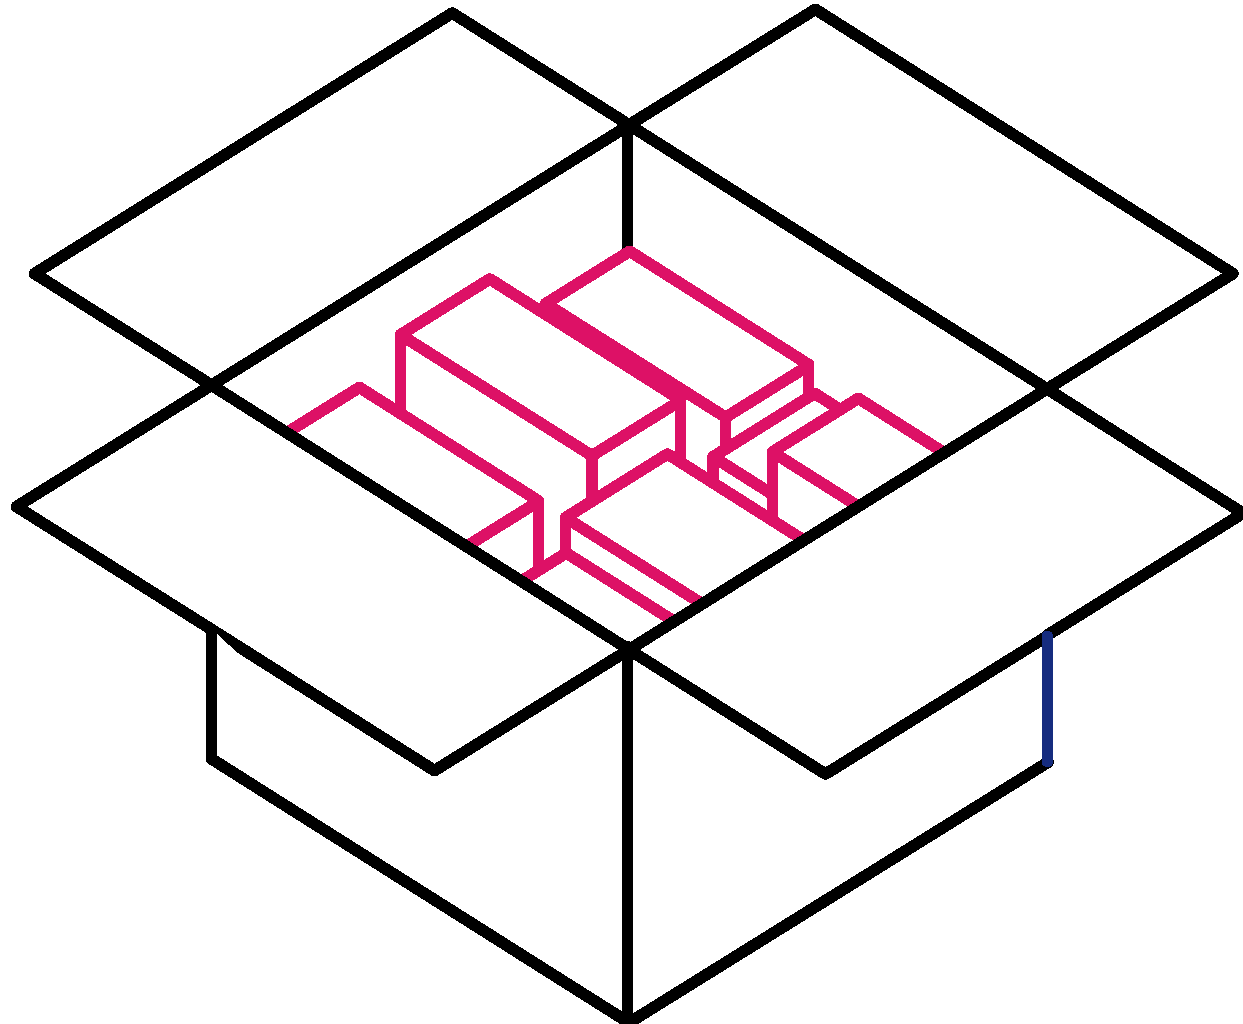
\includegraphics[height=20pt]{../assets/box.pdf}}
\rhead{} %Kopfzeile rechts
\lfoot{} %Fußzeile links
\cfoot{} %Fußzeile mitte
\rfoot{} %Fußzeile rechts
\makeatother


\newcommand{\changefont}{%
    \fontsize{9}{11}\selectfont
}


\setlength\headheight{60pt}
\setlength\footheight{40pt}
%\lfoot{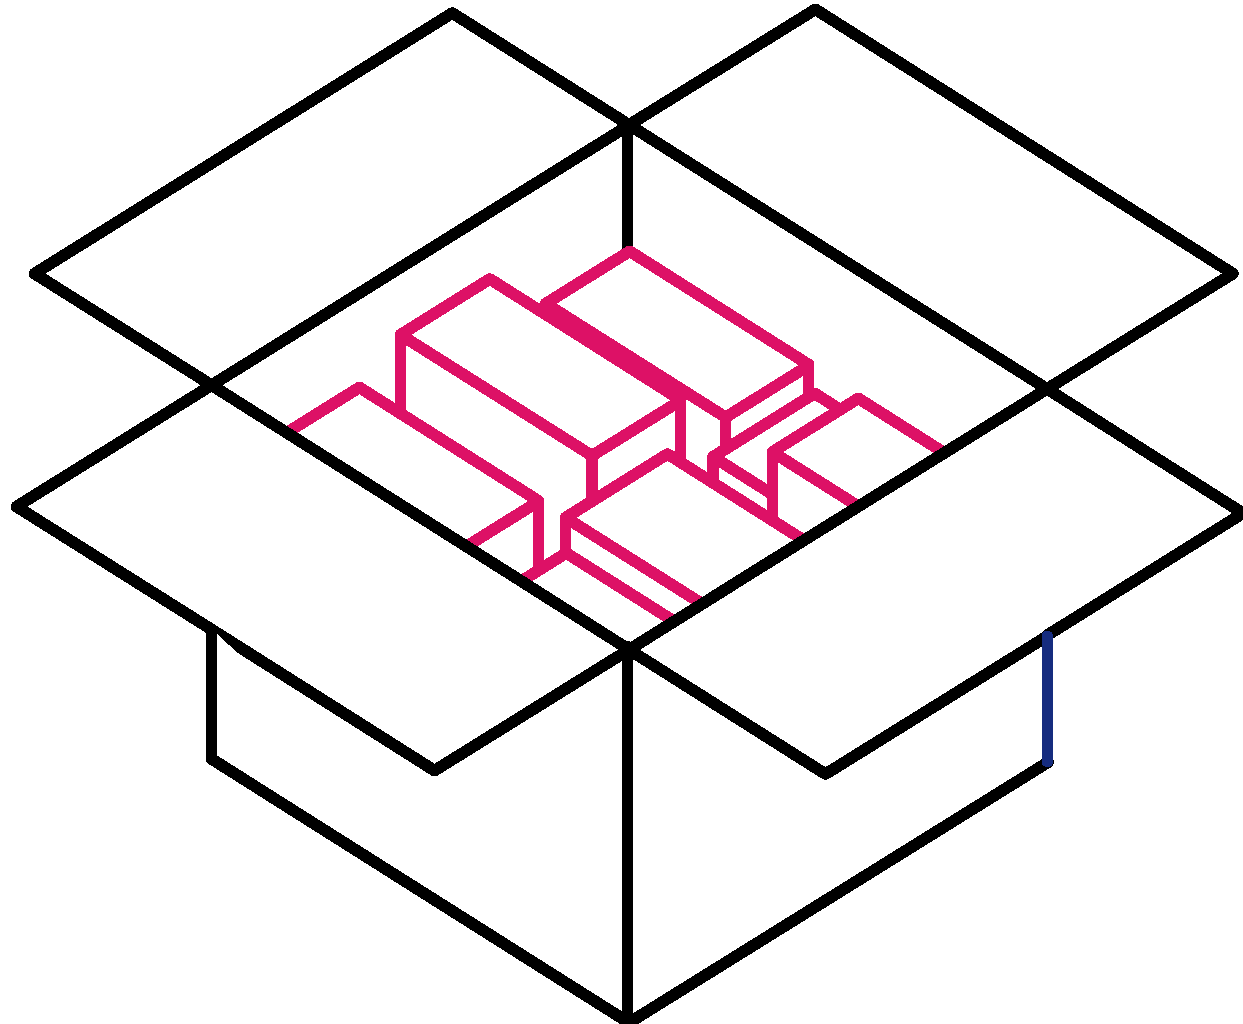
\includegraphics[height=40pt]{../assets/box.pdf}}
\rfoot{\thepage}
\lfoot{\changefont Selbstbericht Medieninformatik\\TH Köln // Institut für Informatik\\ \today}


%\UTF{0192}ndert die Seitennummerierung beim Inhaltsverzeichnis mit eigenem Stil
\renewcommand*{\indexpagestyle}{fancy}
%Verhindert die Seitennummerierung auf den Part-Seiten
\renewcommand*{\partpagestyle}{empty}
%\UTF{0192}ndert die Seitennummerierung bei Chapter mit eigenem Stil
\renewcommand*{\chapterpagestyle}{fancy}

%Abbildungsnummerierung ändern (abhängig von chapter, z.B. Abbildung 1.1)
\renewcommand*{\thefigure}{\thechapter.\arabic{figure}}
%Tabellennummerierung ändern (abhängig von chapter, z.B. Tabelle 1.1)
\renewcommand*{\thetable}{\thechapter.\arabic{table}}

%Paket, um ein Glossar/Abkürzungsverzeichnis anzulegen
\usepackage{nomencl}
\let\abbrev\nomenclature
%Der Name wird in Glossar geändert
\renewcommand{\nomname}{Glossar}
%Definiert die Aufteilung im Glossar zwischen Begriffen und Erläuterung
\setlength{\nomlabelwidth}{.25\hsize}
%Definiert die Punktelinien im Glossar
\renewcommand{\nomlabel}[1]{#1 \dotfill}
\setlength{\nomitemsep}{-\parsep}
%Veranlasst die Erstellung des Glossars
\makenomenclature

%Einrückungen nach Absätzen und Grafiken verhindern
\setlength{\parindent}{0pt}

%Verhindern, dass eine neue Seite für ein einzelnes Wort/Zeile verwendet wird
\clubpenalty = 10000 % schliesst Schusterjungen aus
\widowpenalty = 10000 % schliesst Hurenkinder aus (keine Beleidigung, sondern wirklich ein Fachbegriff)

%Paket für ein deutsches Literaturverzeichnis
\usepackage{bibgerm}

%Paket für die Verwendung von URLs durch den Befehl \url{}
\usepackage{url}

%Paket für Zeilenabstand (onehalfspace, singlespace)
\usepackage{setspace}

%Paket zur Erzeugung von Anführungszeichen durch \enquote{Text}
\usepackage[ngerman]{babel}
\usepackage[babel, german=quotes]{csquotes}

%Paket für farbigen Text
%black,white,green,red,blue,yellow,cyan,magenta
\usepackage{color}

%Paket für farbigen Hintergrund für Verbatim-Umgebung (Quelltext-Umgebung)
\usepackage{fancyvrb}
\usepackage{verbatim,moreverb}
%Grauton für Quelltext-Umgebung definieren 80% Grau
\definecolor{sourcegray}{gray}{.80}
%Paket für Quelltext-Umgebung
\usepackage{listings}

%Paket für Positionierung der Objekte ohne Float (Verwendungsbsp.: \begin{figure}[H])
\usepackage{float}

%Paket zur Erzeugung von Hyperrefs und PDF Informationen
\usepackage[pdftex,plainpages=false,pdfpagelabels,
            pdftitle={ Selbstbericht Medieninformatik // TH Köln // Institut für Informatik},
            pdfauthor={}
            ]{hyperref}

\usepackage{pdfpages}

\providecommand{\tightlist}{%
  \setlength{\itemsep}{0pt}\setlength{\parskip}{0pt}}

\usepackage{tabularx}
\newcolumntype{L}[1]{>{\raggedright\arraybackslash}p{#1}}
\newcolumntype{C}[1]{>{\centering\arraybackslash}p{#1}}
\newcolumntype{R}[1]{>{\raggedleft\arraybackslash}p{#1}}

% URL
\usepackage{hyperref}

% Sonderzeichen
\usepackage{textcomp}
\usepackage{eurosym}

\usepackage{setspace}
\renewcommand{\baselinestretch}{1.2}
\setlength{\parskip}{1em}

\usepackage[sfdefault, light]{roboto}  %% Option 'sfdefault' only if the base font of the document is to be sans serif
%\usepackage[default,osfigures,scale=0.95]{opensans}


\usepackage[raggedright]{titlesec}
\titleformat{\chapter}[display]
  {\normalfont\sffamily\mdseries}
  {\chaptertitlename\ \thechapter}{14pt}{\huge\raggedright}
\titleformat{\section}
  {\normalfont\sffamily\mdseries\LARGE\color{m_pink}\raggedright}
  {\thesection}{1em}{\LARGE}
\titleformat{\subsection}
  {\normalfont\sffamily\mdseries\large\raggedright}
  {\thesubsection}{1em}{\large}

\usepackage[T1]{fontenc}


\usepackage[font=footnotesize]{caption}


% Footer definieren
\makeatletter
\def\footrule{{
  \vskip-\footruleskip\vskip-\footrulewidth
  \color{\footrulecolor}
  \hrule\@width\headwidth\@height
  \footrulewidth\vskip\footruleskip
}}
\makeatother
\renewcommand{\footrulewidth}{0.1pt}
\newcommand{\footrulecolor}{m_green}



\begin{document}

%=== Inhaltsverzeichnis =======================================================
\tableofcontents

%=== Hauptteil =======================================================
%Seitennummerierung des Hauptteils
\mainmatter


\chapter{Human-Computer Interaction}\label{human-computer-interaction}

\section*{Allgemeines:}\label{allgemeines}

Medieninformatik und Mensch-Computer Interaktion stehen in vielerlei
Hinsicht in einem engen Zusammenhang. So beinhaltet etwa der Fachbereich
„Mensch-Computer Interaktion`` der GI e.V. die Fachgruppe
„Medieninformatik`` (siehe auch:
\url{http://fb-mci.gi.de/mensch-computer-interaktion-mci/fachgruppen/medieninformatik.html}).

Im Zusammenhang mit der „third wave of HCI`` (Susan Bødker, 2006 und
2016) wird die aktuelle Bedeutung der Disziplin der Mensch-Computer
Interaktion für die Gestaltung interaktiver System und insbesondere ihre
Rolle für die Medieninformatik deutlich. Nach Bødker besteht eine
aktuelle Herausforderung der 3rd wave of HCI insbesondere darin, dass
sich die Trennlinie von Technologienutzung zwischen
beruflichem/gewerblichem und privatem Bereich mehr und mehr auflöst.
Medieninformatik befasst sich insbesondere mit interaktiven und
multimedialen Systemen in gewerblichen und privaten Nutzungskontexten
und adressiert demnach die Herausforderungen der 3rd wave of HCI.

\section*{Zielsetzungen:}\label{zielsetzungen}

Dieser Schwerpunkt adressiert Kompetenzen, Fähigkeiten und Fertigkeiten
die im Zusammenhang mit der Leitung und dem Management von
Entwicklungsprojekten innovativer, interaktiver Systeme stehen. Dies
umfasst die Nutzungskontexte in verschiedensten Anwendungsbereichen
kritisch zu analysieren, Problemfelder zu identifizieren, Anforderungen
zu spezifizieren, angemessene Vorgehen zur Lösungsentwicklung zu
konzipieren und Gestaltungslösungen zu entwickeln und zu evaluieren.
Absolventen dieses Schwerpunktes arbeiten als UX-Architects, Interaction
Designer oder in Positionen mit ähnlichen Rollenbezeichnungen in
Unternehmen/Institutionen und sind zentrale Entscheidungsträger, wenn es
um die Entwicklung interaktiver Systeme aus Nutzungs -oder
Nutzerperspektive geht.

Neben den vielfältigen weiterentwickelten Kompetenzen (formale,
analytische, methodologische, gestalterische, technologische, etc.)
haben sie die Befähigung zum fachlichen Diskurs vertieft und
implementieren mit ihrer Kommunikationskompetenz eine wichtige
Schnittstelle für die verschiedenen Stakeholder und Gewerke.

\section*{Schwerpunktspezifische
Pflichtmodule}\label{schwerpunktspezifische-pflichtmodule}

\begin{itemize}
\item
  Interaction Design
\item
  Design Methodologies
\item
  Angewandte Statistik für die Mensch-Computer Interaktion
\end{itemize}

\chapter{Multiperspective Product
Development}\label{multiperspective-product-development}

\section*{Zielsetzung:}\label{zielsetzung}

Der Schwerpunkt „Multi-Perspective Product Development'' bereitet die
Studierenden auf die, für viele Projekte der Medieninformatik, typische
Heterogenität vor, welche von der methodologischen über die
technologische bis hin zur soziotechnischen Komponente reicht.
Chakterisierende Merkmale solcher Projekte sind:

\begin{itemize}
\item
  Berücksichtigung von und Kommunikation mit Stakeholdern mit jeweils
  eigenen Perspektiven, die durch ihre Fachsprache, Methoden und
  Techniken sowie entsprechende Fähigkeiten, Verantwortlichkeiten und
  Kompetenzen definiert werden.
\item
  Heterogene soziale, technologische und ökonomische Rahmenbedingungen
  wie z.B.
\item
  die Anwendung von unterschiedlichen, agilen bis hin zu
  „schwergewichtigen'' Vorgehensmodellen,
\item
  lokale Zusammenarbeit in kleinen Teams bis hin zu dezentraler
  Zusammenarbeit in großen, international und interdisziplinär
  aufgestellten Teams,
\item
  ein breites Spektrum der Projektgegenstände von kleinen, nativen Apps
  für mobile Geräte bis hin zu großen, geschäftskritischen,
  internationalisierbaren und responsiven Web-Anwendungen,
\item
  ein breites Spektrum der Projektkontexte von kleinen Inhouse-Projekten
  bis hin zu großen, organisationsübergreifenden internationalen
  Projekten.
\end{itemize}

\section*{Schwerpunktspezifische
Pflichtmodule}\label{schwerpunktspezifische-pflichtmodule-1}

\begin{itemize}
\item
  Privatsphäre \& Sicherheit im Netz
\item
  Visualisierung
\item
  Qualitätssicherung und -management
\end{itemize}

\chapter{Social Computing}\label{social-computing}

\section*{Zielsetzungen:}\label{zielsetzungen-1}

Im Schwerpunkt „Social Computing`` werden die Wechselwirkungen zwischen
Gesellschaft und Informatik in den Mittelpunkt gestellt. Rechnersysteme
und Netzwerke werden von Menschen intentional gestaltet, ausgerichtet an
gesellschaftlichen Normen, Prozessen und Bedürfnissen. Gleichzeitig
beeinflussen IT-Systeme diese gesellschaftlichen Normen und verändern
Prozesse in allen Lebensbereichen. Die verantwortungsbewusste Konzeption
und Realisierung von soziotechnischen Systemen (z.B. Social Software,
Online Communities, e-Health, e-Government und e-Learning Angebote)
sowie die empirische Evaluation existierender Systeme sind zentrale
Ziele. Lösungen sollen unter ganzheitlichen Gesichtspunkten entwickelt
werden. Verschiedene Wertvorstellungen und Interessen unterschiedlicher
Stakeholder müssen identifiziert und berücksichtig werden.

Der Schwerpunkt verbindet daher Theorien, Modelle und Methodik der
Human- und Sozialwissenschaften mit anwendungsorientierter Informatik.
Studierende sollen in der Lage sein, computergestützte Systeme nach
ethischen, politischen, sozialen und psychologischen Kriterien bewerten,
planen und umsetzen zu können.

Ziel ist es, soziale Innovation durch digitale Anwendungen entstehen zu
lassen. Neben den empirischen Methoden werden Designmethoden vermittelt,
sowohl auf der konzeptionellen als auch auf der softwaretechnischen
Implementierungsebene, um robuste, sichere und flexible Systeme zu
gestalten.

\section*{Schwerpunktspezifische
Pflichtmodule}\label{schwerpunktspezifische-pflichtmodule-2}

\begin{itemize}
\item
  Privatsphäre, Vertrauen \& Sicherheit im Netz
\item
  Soziotechnische Entwurfsmuster
\item
  Netzwerk-und Graphentheorie
\end{itemize}

\chapter{Visual Computing}\label{visual-computing}

\section*{Schwerpunktspezifische
Pflichtmodule}\label{schwerpunktspezifische-pflichtmodule-3}

\begin{itemize}
\item
  Storytelling und Narrative Strukturen
\item
  Bildbasierte Computergrafik
\item
  Visualisierung
\end{itemize}

Der Studienschwerpunkt „Visual Computing'' steht an der Schnittstelle
von Computergrafik, Computer Vision, Mensch-Maschine-Kommunikation,
Bild- und Videoverarbeitung, sowie Visualisierung.

Ziel des Studienschwerpunktes Visual Computing ist es, den Studierenden
ein solides Fundament bildbasierter und bildgebender Verfahren zu
vermitteln, indem die Entwicklung praktischer Algorithmen und Programme
anhand ihrer theoretischen Grundlagen erlernt wird. Zusätzlich sollen
die Studierenden in die Lage versetzt werden, die entwickelten
Applikationen zu bewerten, zu präsentieren und auf ihre ethischen
Konsequenzen hin zu prüfen.

Die hohe Interdisziplinarität ist ein Innovationsfaktor und bietet
Schlüsseltechnologien zur Lösung aktueller Problemstellungen in der
Informatik, wie z.B. Virtual Engineering, Visual Analytics, Virtual- und
Augmented Reality, Medizintechnik, Robotik, Animation und Bildsynthese.
Anwendungen des Visual Computing finden sich in den verschiedensten
Bereichen, z.B. in der Unterhaltungsindustrie (Visuelle Effekte,
Computerspiele, Filmindustrie, 360° und 3D Videos), der Medizin
(medizinische Bildverarbeitung, digitale Operationsplanung), der
Automobilindustrie (Fahrerassistenzsysteme), der industriellen Fertigung
(visuelle Qualitätskontrolle), der Internettechnologien und Mobilgeräte
(Remote Rendering, Multimediale Datenbanken, Augmented Reality
Anwendungen) und der digitalen Fotografie.

Um der Interdisziplinarität sowie den unterschiedlichen Ausrichtungen
dieses Studienschwerpunktes gerecht zu werden müssen folgende Module im
Umfang von 18 CP belegt werden:

\begin{itemize}
\item
  Storytelling, Narrative Strukturen
\item
  Bildbasierte Computergrafik
\item
  Visualistik
\end{itemize}

Zudem müssen folgende drei Projekte im Umfang von jeweils 12 cp belegt
werden, die verschiedene Schwerpunkte in diesem heterogenen und schnell
veränderlichen Bereich abdecken:

\begin{itemize}
\item
  Projekt Vision \& Konzept im Studienschwerpunkt Visual Computing
\item
  Projekt Entwicklung im Studienschwerpunkt Visual Computing
\item
  Projekt Forschung im Studienschwerpunkt Visual Computing
\end{itemize}

Weitere 18 CP können aus dem allgemeinen Angebot der Veranstaltungen
aller Kurse aus den Masterstudiengängen Medieninformatik und Informatik
belegt werden, um der Heterogenität der Medieninformatik und des Visual
Computings gerecht zu werden.

\chapter{Weaving the Web}\label{weaving-the-web}

\section*{Zielsetzung:}\label{zielsetzung-1}

Im Studienschwerpunkt „Weaving the Web'' wird die Entwicklung von
Produkten und Diensten im Web in den Mittelpunkt gestellt. Dabei wird
der gesamte Lebenszyklus von der Erarbeitung einer Vision, der
eigentlichen Software Entwicklung bis hin zu der Verwertung als Produkt
und/oder Publikation adressiert.

Als charakterisierende Merkmale für die Entwicklung von Produkten und
Diensten im Web stehen:

\begin{itemize}
\item
  die Einbettung in ein Netz von Prozessen und Informationsflüssen, die
  Dienste, Informationen, Personen und Geräte im Web zusammenfassen,
\item
  der Fokus auf Offenheit, sowohl bei den verwendeten Technologien,
  Frameworks und Plattformen als auch die Haltung in der Kommunikation
  im Team und gegenüber der Community und
\item
  die konsequente Anwendung agiler Vorgehensmodelle sowie die Nutzung
  des Wissens und des kreativen Potentials von Nutzern durch Community
  Managenent.
\end{itemize}

Der Titel der Studienrichtung, „Weaving the Web'' wurde gewählt, da
neben dem klassischen Software Engineering vor allem auch die
Integration eigener Produkte und Dienste in das Web thematisiert wird.

\section*{Schwerpunktspezifische
Pflichtmodule}\label{schwerpunktspezifische-pflichtmodule-4}

\begin{itemize}
\item
  Sicherheit, Privatsphäre und Vertrauen im Netz
\item
  Web Architekturen
\item
  Web Technologien
\end{itemize}

\chapter{Computerethik}\label{computerethik}

\begin{itemize}
\tightlist
\item
  Modulverantwortlich: Prof.~Dr.~Christian Kohls
\item
  Kürzel: CE
\item
  Studiensemester - Wintersemester: 2
\item
  Studiensemester - Sommersemester: 1
\item
  Sprache: deutsch
\item
  Kreditpunkte: 6
\item
  Voraussetzungen nach Prüfungsordnung:
\item
  Typ: Pflichtmodul
\end{itemize}

\section*{Lehrform/SWS:}\label{lehrformsws}

4 SWS: Vorlesung 2 SWS; Seminar 2 SWS

\section*{Arbeitsaufwand:}\label{arbeitsaufwand}

Gesamtaufwand 180 h, davon

\begin{itemize}
\item
  45 h Vorlesung
\item
  90 h Seminar
\item
  45 h Selbststudium
\end{itemize}

\section*{Angestrebte
Lernergebnisse:}\label{angestrebte-lernergebnisse}

Die Studierenden sollen wesentliche Begriffe und Grundpositionen
bezüglich ethischer und sozialer Fragen, die durch die Digitalisierung
in Medien und Gesellschaft (z.B. mediale Kommunikation und der Einsatz
von Informationssystemen) aufgeworfen werden, kennen. Sie sollen
weiterhin Positionen aus wissenschaftlichen Veröffentlichungen in diesem
Bereich erarbeiten, vortragen und dazu Stellung beziehen können.

\section*{Inhalt:}\label{inhalt}

\begin{itemize}
\item
  Ethische Grundbegriffe
\item
  Relativismus, Utilitarismus, Deontologische Theorien
\item
  Ethik für Informatiker*innen
\item
  Professionelle Verantwortung
\item
  Privatsphäre und Datensicherheit
\item
  Ethische Konsequenzen autonomer Systeme
\item
  Potentiale und Gefahren für demokratisches Handeln
\item
  Machtverhältnisse in digitalen Umwelten
\item
  Handlungsfreiheiten in digitalen Systemen
\item
  Quantifizierung von persönlichen Informationen
\item
  Positive Computing
\end{itemize}

\section*{Studien-/Prüfungsleistungen:}\label{studien-pruxfcfungsleistungen}

Abschlusspräsentation und schriftliche Ausarbeitung

\section*{Medienformen:}\label{medienformen}

\begin{itemize}
\item
  Beamer-gestützte Vorlesungen (Folien in elektronischer Form)
\item
  Fallstudien
\item
  Diskussionsrunden
\item
  Anonyme Abstimmungen und Kommentare (PINGO)
\end{itemize}

\section*{Literatur:}\label{literatur}

\begin{itemize}
\item
  Calvo, R. A., \& Peters, D. (2014). Positive computing: Technology for
  wellbeing and human potential.
\item
  Johnson: Computer Ethics, 4rd Edition, Prentice Hall 2007
\item
  Lawrence Lessing: Code Version 2.0 Basic Books, New York 2006
\item
  Himma, Kenneth et al. (eds.): The Handbook of Information and Computer
  Ethics, Wiley
\item
  Spinello, Richard: Case Studies in Information Technology Ethics,
  Prentice Hall
\item
  Capurro, Rafael: Ethik im Netz, Franz Steiner Verlag
\item
  Tavani, Herman: Ethics \& Technology - Ethical Issues in an Age of
  Information and Communication Technology, Wiley
\item
  Wendel, Stephen. (2013). Designing for behavior change: Applying
  psychology and behavioral economics.
\end{itemize}

\chapter{Masterarbeit}\label{masterarbeit}

\begin{itemize}
\tightlist
\item
  Modulverantwortlich: alle Informatik Professoren
\item
  Kürzel: MA
\item
  Studiensemester - Wintersemester: 4
\item
  Studiensemester - Sommersemester: 4
\item
  Sprache: deutsch
\item
  Kreditpunkte: 30
\item
  Voraussetzungen nach Prüfungsordnung: keine
\item
  Typ: Pflichtmodul
\end{itemize}

\section*{Kurzbeschreibung}\label{kurzbeschreibung}

Die Masterarbeit (Master Thesis) und das Kolloquium bilden den Abschluss
des Studiums. Die Masterarbeit ist in der Regel eine eigenständige
Untersuchung mit einer Aufgabenstellung aus der Medieninformatik und
einer ausführlichen Beschreibung und Erläuterung ihrer Lösung. In
fachlich geeigneten Fällen kann sie auch eine schriftliche Hausarbeit
mit fachliterarischem Inhalt sein.

\section*{Lehrform/SWS:}\label{lehrformsws-1}

Eigenständige betreute wissenschaftlich-fachpraktische Arbeit

\section*{Arbeitsaufwand:}\label{arbeitsaufwand-1}

900 Stunden

\section*{Angestrebte
Lernergebnisse:}\label{angestrebte-lernergebnisse-1}

Ziel der Masterarbeit (Master Thesis) und des Kolloquiums ist die
Befähigung, innerhalb einer vorgegebenen Frist eine wissenschaftlich
orientierte Aufgabe aus der Medieninformatik, sowohl in ihren fachlichen
Einzelheiten als auch in den fachübergreifenden Zusammenhängen, nach
wissenschaftlichen, fachpraktischen und gestalterischen Methoden
selbständig zu bearbeiten, zu dokumentieren und zu verteidigen.

\section*{Inhalt:}\label{inhalt-1}

\begin{itemize}
\item
  Die Masterarbeit ist in der Regel eine eigenständige Untersuchung mit
  einer Aufgabenstellung aus der Medieninformatik und einer
  ausführlichen Beschreibung und Erläuterung ihrer Lösung.
\item
  In fachlich geeigneten Fällen kann sie auch eine schriftliche
  Hausarbeit mit fachliterarischem Inhalt sein.
\item
  Konkrete Inhalte je nach Thema.
\end{itemize}

\section*{Studien-/Prüfungsleistungen:}\label{studien-pruxfcfungsleistungen-1}

\begin{itemize}
\item
  Masterarbeit: Dokumentation der geleisteten Arbeit mit Zielsetzung und
  Aufgabenstellung, Stand von Wissenschaft und Technik, verwendeten
  Problemlösungsmethoden, erzielten Resultaten, offenen Fragen,
  Reflektion, verwendeten Quellen etc..
\item
  Kolloquium: Darstellung und Verteidigung der Arbeit und der
  wichtigsten Ergebnisse im Rahmen eines Vortrages mit anschließender
  Diskussion
\item
  Bearbeitungszeiten siehe Prüfungsordnung
\end{itemize}

\section*{Medienformen:}\label{medienformen-1}

Je nach Thema

\section*{Literatur:}\label{literatur-1}

Je nach Thema

\chapter{Spezielle Gebiete der
Mathematik}\label{spezielle-gebiete-der-mathematik}

\begin{itemize}
\tightlist
\item
  Modulverantwortlich: Prof.~Dr.~Wolfgang Konen, Prof.~Dr.~Boris Naujoks
\item
  Kürzel: SGM-D
\item
  Studiensemester - Wintersemester: 1
\item
  Studiensemester - Sommersemester: 2
\item
  Sprache: deutsch
\item
  Kreditpunkte: 6
\item
  Voraussetzungen nach Prüfungsordnung: Keine über die
  Zulassungsvorrausetzungen zum Studium hinausgehenden
\item
  Typ: Pflichtmodul
\end{itemize}

\section*{Kurzbeschreibung}\label{kurzbeschreibung-1}

Es werden Grundlagen für die Analyse und algorithmische Verarbeitung von
Graph basierten Daten eingeführt.

\section*{Lehrform/SWS:}\label{lehrformsws-2}

4 SWS: Vorlesung 2 SWS; Seminar 2 SWS

\section*{Arbeitsaufwand:}\label{arbeitsaufwand-2}

Gesamtaufwand 150 h, davon

\begin{itemize}
\item
  30 h Vorlesung
\item
  30 h Seminar
\item
  12 h Selbststudium
\end{itemize}

\section*{Angestrebte
Lernergebnisse:}\label{angestrebte-lernergebnisse-2}

Mathematische Abstraktion und Fertigkeiten sind unverzichtbare
Grundlagen wissenschaftlichen Arbeitens im Bereich der Informatik. Durch
den Besuch dieser Veranstaltung sollen Studierende ihre
mathematisch-abstrakte Analysefähigkeit weiter ausbauen, ihre Sicherheit
im Umgang mit mathematischen Methoden mit Relevanz für die Informatik
stärken, die Fähigkeit zur selbständigen Einarbeitung in neue
mathematische Sachverhalte erhalten und ihre Beurteilungsfähigkeit im
Umgang mit mathematisch-abstrakten Themen erhöhen.

\section*{Inhalt:}\label{inhalt-2}

Exemplarische Fragestellungen der Mathematik in der Informatik mit
beispielhaften Themen wie:

\begin{itemize}
\item
  Deskriptive Statistik, Datenanalyse, Visualisierung
\item
  Schließende Statistik, Trendanalyse
\item
  Prädikatenlogik
\item
  gemischt-ganzzahlige Optimierung
\item
  Simulationsverfahren
\item
  Differentialgleichung und ihre numerische Lösung
\end{itemize}

\section*{Studien-/Prüfungsleistungen:}\label{studien-pruxfcfungsleistungen-2}

Präsentation und Klausur

\section*{Medienformen:}\label{medienformen-2}

Präsentationsmaterialien, Arbeitsblätter

\section*{Literatur:}\label{literatur-2}

\begin{itemize}
\item
  Liu, Eric Zhi-Feng, e.a., Web-based Peer Review: The learner as both
  Adapter and Reviewer, IEEE Transactions on Education, Vol 44, No 3,
  August 2001
\item
  Tufte, E.R., The Visual Display of Quantitative Information,
  Cheshire,CT, Graphics Press 1983
\item
  Hanke-Bourgeois, M., Grundlagen der Numerischen Mathematik und des
  Wissenschaftlichen Rechnens, 2. Aufl., Teubner 2006.
\item
  Siehe ILIAS Modul MAS \& SGM, Dokument Allgemeine Hinweise
\end{itemize}

\chapter{Schwerpunktmodul 1}\label{schwerpunktmodul-1}

\begin{itemize}
\tightlist
\item
  Modulverantwortlich: alle Informatik Professoren
\item
  Kürzel: SPM1
\item
  Studiensemester - Wintersemester: 1
\item
  Studiensemester - Sommersemester: 2
\item
  Sprache: deutsch
\item
  Kreditpunkte: 6
\item
  Voraussetzungen nach Prüfungsordnung: keine
\item
  Typ: Wahlpflichtmodul
\end{itemize}

\section*{Arbeitsaufwand:}\label{arbeitsaufwand-3}

180 Stunden

\chapter{Schwerpunktmodul 2}\label{schwerpunktmodul-2}

\begin{itemize}
\tightlist
\item
  Modulverantwortlich: alle Informatik Professoren
\item
  Kürzel: SPM2
\item
  Studiensemester - Wintersemester: 1
\item
  Studiensemester - Sommersemester: 2
\item
  Sprache: deutsch
\item
  Kreditpunkte: 6
\item
  Voraussetzungen nach Prüfungsordnung: keine
\item
  Typ: Wahlpflichtmodul
\end{itemize}

\section*{Arbeitsaufwand:}\label{arbeitsaufwand-4}

180 Stunden

\chapter{Schwerpunktmodul 3}\label{schwerpunktmodul-3}

\begin{itemize}
\tightlist
\item
  Modulverantwortlich: alle Informatik Professoren
\item
  Kürzel: SPM3
\item
  Studiensemester - Wintersemester: 2
\item
  Studiensemester - Sommersemester: 1
\item
  Sprache: deutsch
\item
  Kreditpunkte: 6
\item
  Voraussetzungen nach Prüfungsordnung: keine
\item
  Typ: Wahlpflichtmodul
\end{itemize}

\section*{Arbeitsaufwand:}\label{arbeitsaufwand-5}

180 Stunden

\chapter{Wahlpflichtmodul 1}\label{wahlpflichtmodul-1}

\begin{itemize}
\tightlist
\item
  Modulverantwortlich: alle Informatik Professoren
\item
  Kürzel: WPM
\item
  Studiensemester - Wintersemester: 3
\item
  Studiensemester - Sommersemester: 3
\item
  Sprache: deutsch
\item
  Kreditpunkte: 6
\item
  Voraussetzungen nach Prüfungsordnung: keine
\item
  Typ: Pflichtmodul
\end{itemize}

\section*{Arbeitsaufwand:}\label{arbeitsaufwand-6}

180 Stunden

\chapter{Wahlpflichtmodul 2}\label{wahlpflichtmodul-2}

\begin{itemize}
\tightlist
\item
  Modulverantwortlich: alle Informatik Professoren
\item
  Kürzel: WPM
\item
  Studiensemester - Wintersemester: 3
\item
  Studiensemester - Sommersemester: 3
\item
  Sprache: deutsch
\item
  Kreditpunkte: 6
\item
  Voraussetzungen nach Prüfungsordnung: keine
\item
  Typ: Pflichtmodul
\end{itemize}

\section*{Arbeitsaufwand:}\label{arbeitsaufwand-7}

180 Stunden

\chapter{Wahlpflichtmodul 3}\label{wahlpflichtmodul-3}

\begin{itemize}
\tightlist
\item
  Modulverantwortlich: alle Informatik Professoren
\item
  Kürzel: WPM
\item
  Studiensemester - Wintersemester: 3
\item
  Studiensemester - Sommersemester: 3
\item
  Sprache: deutsch
\item
  Kreditpunkte: 6
\item
  Voraussetzungen nach Prüfungsordnung: keine
\item
  Typ: Pflichtmodul
\end{itemize}

\section*{Arbeitsaufwand:}\label{arbeitsaufwand-8}

180 Stunden

\chapter{Research Methods}\label{research-methods}

\begin{itemize}
\tightlist
\item
  Modulverantwortlich: Prof.~Dr.~Gerhard Hartmann
\item
  Kürzel: RM
\item
  Studiensemester - Wintersemester: 2
\item
  Studiensemester - Sommersemester: 1
\item
  Sprache: deutsch
\item
  Kreditpunkte: 6
\item
  Voraussetzungen nach Prüfungsordnung:
\item
  Typ: Pflichtmodul
\end{itemize}

\section*{Lehrform/SWS:}\label{lehrformsws-3}

6 SWS: Vorlesung 2 SWS; Übung 2SWS; Projekt 3 SWS

\section*{Arbeitsaufwand:}\label{arbeitsaufwand-9}

Gesamtaufwand 180 h, davon

\begin{itemize}
\item
  45 h Vorlesung
\item
  30 h Übung
\item
  105 h Projekt
\end{itemize}

\section*{Angestrebte
Lernergebnisse:}\label{angestrebte-lernergebnisse-3}

Die Teilnehmer sind in der Lage verschiedene methodische Rahmen für die
Beantwortung empirischer Problem- oder Fragestellungen zu benennen,
kritisch einzuordnen und für ihre konkreten Projekte (Zielsetzungen,
Rahmenbedingungen, etc.) eine rational begründete Wahl eines (oder einer
Kombination aus verschiedenen) methodischen Rahme zu treffen und zu
kommunizieren.

Sie sind in der Lage, die Methoden projektgerecht und methodenkompetent
anzuwenden und Resultate angemessen zu interpretieren und

kritisch zu diskutieren..

\section*{Inhalt:}\label{inhalt-3}

\begin{itemize}
\item
  Forschungsdesign und -planung
\item
  quantitative und qualitative Methoden
\item
  empirische und analytische Ansätze
\item
  in-vivo vs.~in-vitro Rahmenbedinungen bei empirischen Methoden
\item
  Datenweiterverarbeitung und Ergebnisinterpretation und -präsentation
\end{itemize}

\section*{Studien-/Prüfungsleistungen:}\label{studien-pruxfcfungsleistungen-3}

schriftliche Modulprüfung

\section*{Medienformen:}\label{medienformen-3}

\begin{itemize}
\item
  beamergestützte Vorlesung
\item
  E-Books
\end{itemize}

\section*{Literatur:}\label{literatur-3}

\begin{itemize}
\item
  Bortz, J.; Döring, N.: „Forschungsmethoden und Evaluation für Human-
  und Sozialwissenschaftler``, Springer Heidelberg, Berlin, 2006
\item
  Lazar, J. Feng, J., Hochheiser, H.: ``Research Methods in
  Human-Computer Interaction'', Wiley, 2009
\item
  May, G., Mruck, K.: ``Handbuch Qualitative Forschung in der
  Psychologie, Springer, 2010
\end{itemize}

\chapter{Design Methodologies}\label{design-methodologies}

\begin{itemize}
\tightlist
\item
  Modulverantwortlich: Prof.~Dr.~Gerhard Hartmann, Prof.~Dr.~Christian
  Kohls
\item
  Kürzel: DM
\item
  Studiensemester - Wintersemester: 1
\item
  Studiensemester - Sommersemester: 2
\item
  Sprache: deutsch
\item
  Kreditpunkte: 6
\item
  Voraussetzungen nach Prüfungsordnung:
\item
  Typ: Schwerpunktmodul
\end{itemize}

\section*{Lehrform/SWS:}\label{lehrformsws-4}

6 SWS: Vorlesung 2 SWS; Übung 1 SWS; Projekt 3 SWS

\section*{Arbeitsaufwand:}\label{arbeitsaufwand-10}

Gesamtaufwand 180 h, davon

\begin{itemize}
\item
  45 h Vorlesung
\item
  30 h Übung
\item
  105 h Projekt
\end{itemize}

\section*{Angestrebte
Lernergebnisse:}\label{angestrebte-lernergebnisse-4}

Die Teilnehmer sind in der Lage verschiedene methodische Rahmen für die
Gestaltung interaktiver Systeme zu benennen, kritisch einzuordnen und
für ihre konkreten Projekte eine rational begründete Wahl eines (oder
einer Kombination aus verschiedenen) methodischen Rahmen zu treffen und
zu kommunizieren. Sie sind in der Lage, die Methoden projektgerecht und
kompetent anzuwenden und Design-Entscheidungen und „trade-offs`` zu
begründen sowie Designresultate unter Einbeziehung der Designmethoden
kritisch zu diskutieren.

\section*{Inhalt:}\label{inhalt-4}

\begin{itemize}
\item
  Gestaltungstheorien
\item
  Menschzentrierte Gestaltung (human-centered design)
\item
  Nutzungszentrierte Gestaltung (usage-centered design)
\item
  Wertebezogene Gestaltungsansätze
\item
  Gestaltungsprinzipien
\item
  Gestaltungsmuster
\item
  Partizipatives Design
\item
  Design Thinking
\end{itemize}

\section*{Studien-/Prüfungsleistungen:}\label{studien-pruxfcfungsleistungen-4}

Mündliche Prüfung

\section*{Medienformen:}\label{medienformen-4}

\begin{itemize}
\item
  Beamer-gestützte Vorlesungen
\item
  Lehrfilme
\item
  E-Books
\item
  Präsentationsmaterialien
\end{itemize}

\section*{Literatur:}\label{literatur-4}

\begin{itemize}
\item
  Borchers: ``A Pattern Approach to Interaction Design'', Wiley \& Sons,
  2001
\item
  Brown: ``Change by Design: How Design Thinking Transforms
  Organizations and Inspires Innovation``, Harper Business, 2009
\item
  ISO 9241, Teil 110, Grundsätze der Dialoggestaltung
\item
  ISO 9241, Teil 210, Human-centered Design for interactive Systems
\item
  Constantine \& Lockwood: ``Software for Use, A Practical Guide to the
  Models and Methods of Usage-Centered Design``, Addison Wesley, 1999
\item
  Schweppenhäuser: ``Designtheorie'', Springer, 2016
\item
  Martin, Hanington: ``Designmethoden .100 Recherchemethoden und
  Analysetechniken für erfolgreiche Gestaltung``, Stiebner, 2013
\end{itemize}

\chapter{Interaction Design}\label{interaction-design}

\begin{itemize}
\tightlist
\item
  Modulverantwortlich: Prof.~Dr.~Gerhard Hartmann
\item
  Kürzel: ID
\item
  Studiensemester - Wintersemester: 1
\item
  Studiensemester - Sommersemester: 2
\item
  Sprache: deutsch
\item
  Kreditpunkte: 6
\item
  Voraussetzungen nach Prüfungsordnung:
\item
  Typ: Schwerpunktmodul
\end{itemize}

\section*{Lehrform/SWS:}\label{lehrformsws-5}

6 SWS: Vorlesung 2 SWS; Übung 1 SWS; Projekt 3 SWS

\section*{Arbeitsaufwand:}\label{arbeitsaufwand-11}

Gesamtaufwand 180 h, davon

\begin{itemize}
\item
  45 h Vorlesung
\item
  30 h Übung
\item
  105 h Projekt
\end{itemize}

\section*{Angestrebte
Lernergebnisse:}\label{angestrebte-lernergebnisse-5}

Ziel ist vor allem, die Benutzerperspektive im Entwicklungsprozess
interaktiver Systeme zu berücksichtigen, nicht von der Technologie
sondern von menschlichen Erfordernissen auszugehen und eine
entsprechende Interaktionsmodellierung und --gestaltung erreichen zu
können. Dabei wird besonderer Wert auf den Auf- bzw. Ausbau von
Entwurfskompetenz („reflection in action``, „conversation with the
material``) gelegt, die das systematische Entwickeln von
Gestaltungsalternativen, deren Bewertung, der Synthese gefundener
Qualitäten in kohärenten und konsistenten Systementwürfen und den
systematischen, konstruktiven Umgang mit trade-offs und ein insgesamt
iteratives Vorgehen beinhaltet.

Die Studierenden haben konzeptionelles Design (Conceptual Design)
verstanden, können es souverän anwenden und als Vorgehen kritisch
einordnen, um aufgabenangemessene und aus Benutzersicht angenehme
Technologienutzung zu gestalten. Die Studierenden haben den Ansatz
„Designing for Life'' verstanden und wissen, wie sie dies methodisch
umsetzen können.

\section*{Inhalt:}\label{inhalt-5}

\begin{itemize}
\item
  Analyse und Dokumentation menschlichen, situierten Handelns
\item
  Entwicklung präskriptiver Handlungsmodelle
\item
  Analyse und kritische Einordnung präskriptiver Handlungsmodelle
\item
  Konzeptuelles Design
\item
  Interaktionskonzeption und -gestaltung
\item
  Sketching und Prototyping Techniken
\item
  Case Studies
\item
  Evaluationsmethoden und --techniken
\end{itemize}

\section*{Studien-/Prüfungsleistungen:}\label{studien-pruxfcfungsleistungen-5}

schriftliche Ausarbeitung und Designartefakte

\section*{Medienformen:}\label{medienformen-5}

\begin{itemize}
\item
  Beamer-gestützte Vorlesungen
\item
  Lehrfilme
\item
  Präsentationsmaterialien
\end{itemize}

\section*{Literatur:}\label{literatur-5}

\begin{itemize}
\item
  Winograd, Terry (ed.), Bringing Design to Software, Addison Wesley,
  1996, ISBN: 0-201-85491-0
\item
  Courage, Cathrine; Baxter, Kathy, „Understanding Your Users``. A
  practical guide to user requirements. Methods, Tools, \& Techniques,
  Kaufman Morgan Publishers, Elsevier, 2005, ISBN: 1-55860-935-0
\item
  Dix, Allan; Filay, Janet; Abowd Gregory D.; Beale, Russel,
  Human-Computer Interaction, 3rd. edition, Pearson Prentice Hall, 2004,
  ISBN: 0130-461091
\item
  Preece, Jenny; Rogers, Yvonne; Sharp, Helen, Interaction Design,
  beyond human-computer interaction, John Wiley \& Sons, Inc., New York,
  ISBN: 0-471-49278-7
\item
  Pruitt, John; Adlin Tamara, „The Persona Lifecycle``. Keeping People
  in Mind Troughout Product Design, Morgan Kaufman Publishers, Elsevier,
  2006. ISBN: 13- 978-0-12-566251-2
\item
  Raskin, J., The Human Interface, Addison Wesley, 2000, ISBN:
  0-201-37937-6
\item
  Solso, Robert, L.; MacLin, M. Kimberley; MacLin, Otto, H., Cognitive
  Psychology, Pearson International Edition, Seventh Ed., 2005, ISBN:
  0-205-41030-8
\item
  Cooper, Alan und Reimann Robert, Cronin, David: „About Face 3.0``, The
  Essentials of Interaction Design, Wiley, 2007. ISBN: 0470084111
\item
  Snyder, Carolyn, „Paper Prototyping``, Morgan Kaufman Publishers,
  2003, ISBN: 1-55860-870-2
\item
  Bortz, J.; Döring, N., Forschungsmethoden und Evaluation für Human-
  und Sozialwissenschaftler, Springer Heidelberg, Berlin, 2006
\end{itemize}

\chapter{Angewandte Statistik für die Mensch-Computer
Interaktion}\label{angewandte-statistik-fuxfcr-die-mensch-computer-interaktion}

\begin{itemize}
\tightlist
\item
  Modulverantwortlich: Prof.~Dr.~Gerhard Hartmann
\item
  Kürzel: Stat
\item
  Studiensemester - Wintersemester: 2
\item
  Studiensemester - Sommersemester: 1
\item
  Sprache: deutsch
\item
  Kreditpunkte: 6
\item
  Voraussetzungen nach Prüfungsordnung:
\item
  Typ: Schwerpunktmodul
\end{itemize}

\section*{Lehrform/SWS:}\label{lehrformsws-6}

Vorlesung; Übung

\begin{verbatim}

Angaben zu SWS fehlen
\end{verbatim}

\section*{Arbeitsaufwand:}\label{arbeitsaufwand-12}

Gesamtaufwand 180 h, davon

\begin{itemize}
\item
  45 h Vorlesung
\item
  30 h Übung
\item
  105 h Selbststudium
\end{itemize}

\section*{Angestrebte
Lernergebnisse:}\label{angestrebte-lernergebnisse-6}

Die Studierenden sind in der Lage empirische Daten so darzustellen, dass
wesentlichen Strukturen erkennbar sind. Die Studierenden können
angemessene Kennzahlen und Verfahren zur Charakterisierung von
empirischen Daten spezifizieren und ermitteln. Sie beherrschen
wesentliche Konzepte zur Visualisierung von empirischen Daten und können
erste (explorative) Analysen durchführen.

Die Studierenden kennen grundlegende Konzepte und Verfahren der
Inferenzstatistik. Sie sind in der Lage, empirische Daten zu
analysieren, Hypothesen zu testen und die Ergebnisse hinsichtlich
empirischer Fragestellungen zu interpretieren. Sie können Gütekriterien
zur Auswahl unterschiedlicher Verfahren benennen und anwenden.

\section*{Inhalt:}\label{inhalt-6}

Merkmale und Skalen, univariante Häufigkeitsverteilungen, Lagemaße,
Streuung und Schiefe, Konzentration, bivariate Häufigkeitsverteilungen
und Kontingenz, Korrelations- und Regressionsanalyse, Verhältnis -- und
Indexzahlen.

Diskrete und Stetige Zufallsvariablen, Population und
Parameterschätzung, Hypothesentests und Signifikanz, t-Tests,

Konfidenzintervalle, Fehlertypen, Effektstärken und Power, multivariate
Verfahren (ein- und mehrfaktorielle Varianzanalysen und entsprechendes
Forschungsdesign).

\section*{Studien-/Prüfungsleistungen:}\label{studien-pruxfcfungsleistungen-6}

Übungsaufgaben und schriftliche Modulprüfung

\section*{Medienformen:}\label{medienformen-6}

\begin{itemize}
\tightlist
\item
  Beamer-gestützte Vorlesungen (Vorlesungschrift mittels tablet) und
  Übungsaufgaben
\end{itemize}

\section*{Literatur:}\label{literatur-6}

\begin{itemize}
\item
  Statistik für Human- und Sozialwissenschaftler''; J. Bortz und C.
  Schuster, Springer, 2010
\item
  ``Modern Staistical Methods for HCI'', Judy Robertson, Maurits Kaptein
  (Eds), Springer, 2016
\item
  ``Deskriptive Statistik''; R. Kosfeld, H. Eckey, M. Türck; Springer,
  2016
\item
  ``Inferenzstatistik verstehen''; M. Janczyk, R. Pfister, Springer,
  2013
\end{itemize}

\chapter{Sketching and Designing for User
Experience}\label{sketching-and-designing-for-user-experience}

\begin{itemize}
\tightlist
\item
  Modulverantwortlich: Prof.~Dr.~Gerhard Hartmann
\item
  Kürzel: SUE
\item
  Studiensemester - Wintersemester: 1
\item
  Studiensemester - Sommersemester: 2
\item
  Sprache: deutsch
\item
  Kreditpunkte: 6
\item
  Voraussetzungen nach Prüfungsordnung:
\item
  Typ: Wahlpflichtmodul
\end{itemize}

\section*{Lehrform/SWS:}\label{lehrformsws-7}

6 SWS: Vorlesung 2 SWS; Übung 1 SWS; Projekt 3 SWS

\section*{Arbeitsaufwand:}\label{arbeitsaufwand-13}

Gesamtaufwand 180 h, davon

\begin{itemize}
\item
  45 h Vorlesung
\item
  30 h Übung
\item
  105 h Projekt
\end{itemize}

\section*{Angestrebte
Lernergebnisse:}\label{angestrebte-lernergebnisse-7}

Die Studierenden sind in der Lage de- und präskriptiv Nutzer- oder deren
nutzungsbezogene Sachverhalte oder Situationen mit einem umfänglichen
Vokabular visuell-graphisch adäquat für verschiedene Stakeholder
auszudrücken.

\section*{Inhalt:}\label{inhalt-7}

\begin{itemize}
\item
  User Experience Modelle
\item
  Sketching Techniken
\item
  Storyboards
\item
  Empathy maps
\item
  Prototyping
\end{itemize}

\section*{Studien-/Prüfungsleistungen:}\label{studien-pruxfcfungsleistungen-7}

Projektpräsentationsprüfung

\section*{Medienformen:}\label{medienformen-7}

\begin{verbatim}

Bitte noch ergänzen
\end{verbatim}

\section*{Literatur:}\label{literatur-7}

\begin{itemize}
\item
  Bill Buxton ``Sketching User Experience'', Focal Press, 2007
\item
  Saul Greenberg, Bill Buxton et al. ``Sketching User Experiences: The
  workbook'', Elsevier, 2012
\item
  Snyder, Carolyn, „Paper Prototyping``, Morgan Kaufman Publishers, 2003
\end{itemize}

\chapter{Projektarbeit - Entwicklung im Kontext des
Studienschwerpunkts}\label{projektarbeit---entwicklung-im-kontext-des-studienschwerpunkts}

\begin{itemize}
\tightlist
\item
  Modulverantwortlich: Prof.~Dr.~Kristian Fischer, Prof.~Dr.~Mario
  Winter, Prof.~Hans Kornacher, Prof.~Dr.~Martin Eisemann,
  Prof.~Dr.~Christian Kohls, Prof.~Dr.~Gerhard Hartmann
\item
  Kürzel: WTWP-E
\item
  Studiensemester - Wintersemester: 2
\item
  Studiensemester - Sommersemester: 3
\item
  Sprache: deutsch
\item
  Kreditpunkte: 12
\item
  Voraussetzungen nach Prüfungsordnung: keine
\item
  Typ: Schwerpunktprojekt
\end{itemize}

\section*{Kurzbeschreibung}\label{kurzbeschreibung-2}

In einem Projekt wird, basierend auf einem existierenden Konzept, ein
„minimal viable Prototype`` entwickelt

\section*{Lehrform/SWS:}\label{lehrformsws-8}

Projektarbeit

\section*{Arbeitsaufwand:}\label{arbeitsaufwand-14}

360 Stunden

\section*{Angestrebte
Lernergebnisse:}\label{angestrebte-lernergebnisse-8}

Die Studentinnen und Studenten

\begin{itemize}
\item
  können, basierend auf einem dokumentierten Konzept einen „minimal
  viable Prototype`` entwickeln
\item
  kennen Projektmanagement Techniken und Prozesse und können Sie auf ihr
  Projekt anwenden
\item
  kennen Qualitätskriterien für Code, können Code auf dieser Basis
  analysieren und können die Kriterien in Ihrer Entwicklung erfüllen
\end{itemize}

\section*{Inhalt:}\label{inhalt-8}

Das Projekt gliedert sich in zwei Teile:

\begin{itemize}
\item
  In der eigentlichen Projektarbeit wird der Prototyp entwickelt
\item
  In dem Teil „Advanced Seminar`` wird die Recherche durchgeführt. Es
  werden Analysetechniken für die Bewertung von kommerziellen Lösungen
  angewandt. Hierbei kann es sich sowohl um Konkurrenzprodukte handeln
  als auch um Dienste oder Frameworks, auf die das Produkt aufbauen
  könnte. Als Schwerpunkt dieses Teils werden wissenschaftliche Felder
  identifiziert, die Input und für das Produkt liefern können, es werden
  relevante Ergebnisse ermittelt und in einem wissenschaftlichen Seminar
  diskutiert.
\end{itemize}

\section*{Studien-/Prüfungsleistungen:}\label{studien-pruxfcfungsleistungen-8}

Projektarbeit

\section*{Medienformen:}\label{medienformen-8}

n/a

\chapter{Projektarbeit - Assessment/Evaluation, Forschung und Verwertung
im Kontext des
Studienschwerpunkts}\label{projektarbeit---assessmentevaluation-forschung-und-verwertung-im-kontext-des-studienschwerpunkts}

\begin{itemize}
\tightlist
\item
  Modulverantwortlich: Prof.~Dr.~Kristian Fischer, Prof.~Dr.~Mario
  Winter, Prof.~Dr.~Martin Eisemann, Prof.~Dr.~Christian Kohls,
  Prof.~Dr.~Gerhard Hartmann
\item
  Kürzel: WTWP-V
\item
  Studiensemester - Wintersemester: 3
\item
  Studiensemester - Sommersemester: 1
\item
  Sprache: deutsch
\item
  Kreditpunkte: 12
\item
  Voraussetzungen nach Prüfungsordnung: keine
\item
  Typ: Schwerpunktprojekt
\end{itemize}

\section*{Kurzbeschreibung}\label{kurzbeschreibung-3}

Auf Basis eines bereits ausgearbeiteten Prototypen werden in diesem
Modul die Schritte Deployment, Qualitätssicherung, Kontinuierliche
Integration sowie Produktmanagement und -marketing geplant, durchgeführt
und kritisch reflektiert.

\section*{Lehrform/SWS:}\label{lehrformsws-9}

Projektarbeit

\section*{Arbeitsaufwand:}\label{arbeitsaufwand-15}

360 Stunden

\section*{Angestrebte
Lernergebnisse:}\label{angestrebte-lernergebnisse-9}

Die Studentinnen und Studenten können die Kernfunktionen eines Produktes
identifizieren und sind in der Lage einen Prototypen als minimal viable
product in den Markt oder die Community zu bringen.

Die Teilnehmer kennen Deployment Strategien, Konzepte und Techniken der
Kontinuierlichen Integration und können diese in einem spezifischen
Projektkontext anwenden.

Die Studierenden sind in der Lage eine Produkt Management Strategie für
ein Online Produkt zu entwickeln und zu implementieren. Alternativ
können die Studierenden die gewonnen Erkenntnisse aus dem Produkt in der
Community z.B. in Form eines Konferenzbeitrags sichtbar machen und einen
wissenschaftlichen Diskurs dazu führen.

\section*{Inhalt:}\label{inhalt-9}

In der eigentlichen Projektarbeit wird ein fertiger, lauffähiger
Prototyp evaluiert und in Form eines minimal viable product zugänglich
gemacht. Im Rahmen des Moduls wird eine Produktmanagement Strategie
entwickelt und das Produkt wird unter Qualitätsmanagement
Gesichtspunkten beleuchtet.

Variante: In der eigentlichen Projektarbeit wird ein fertiger,
lauffertiger Prototyp evaluiert und in Form eines minimal viable product
zugänglich gemacht. Im Rahmen des Projekts werden Konzepte und Techniken
der Kontinuierlichen Integration auf das minimal viable product
angewendet.

Zur Unterstützung werden Workshops/Seminare in den Bereichen Produkt
Management, Web Deployment und Continuous Integration angeboten.

\section*{Studien-/Prüfungsleistungen:}\label{studien-pruxfcfungsleistungen-9}

Projektarbeit

\section*{Medienformen:}\label{medienformen-9}

n/a

\chapter{Projektarbeit - Vision und Konzept im Kontext des
Studienschwerpunkts}\label{projektarbeit---vision-und-konzept-im-kontext-des-studienschwerpunkts}

\begin{itemize}
\tightlist
\item
  Modulverantwortlich: Prof.~Dr.~Kristian Fischer, Prof.~Dr.~Mario
  Winter, Prof.~Dr.~Martin Eisemann, Prof.~Dr.~Christian Kohls,
  Prof.~Dr.~Gerhard Hartmann
\item
  Kürzel: WTWP-VK
\item
  Studiensemester - Wintersemester: 1
\item
  Studiensemester - Sommersemester: 2
\item
  Sprache: deutsch
\item
  Kreditpunkte: 12
\item
  Voraussetzungen nach Prüfungsordnung: keine
\item
  Typ: Schwerpunktprojekt
\end{itemize}

\section*{Kurzbeschreibung}\label{kurzbeschreibung-4}

In einem Projekt wird eine Idee für ein Produkt oder einen Dienst
entwickelt, eine Recherche des Marktes und Standes des
wissenschaftlichen Wissens durchgeführt, und ein Konzept soweit
definiert und dokumentiert, dass in einem nachfolgenden Schritt ein
Entwicklerteam in der Lage ist, einen ersten Prototyp zu realisieren.

\section*{Lehrform/SWS:}\label{lehrformsws-10}

Projektarbeit

\section*{Arbeitsaufwand:}\label{arbeitsaufwand-16}

360 Stunden

\section*{Angestrebte
Lernergebnisse:}\label{angestrebte-lernergebnisse-10}

Die Studentinnen und Studenten

\begin{itemize}
\item
  können Kreativitätstechniken anwenden um zu Produktideen zu kommen
\item
  können zu einem kritischen Fachdiskurs über Potenziale und Risiken der
  Ideen beitragen
\item
  können wissenschaftliche Gebiete, die für das Produkt wesentlich sein
  können, identifizieren, den Stand des Wissens ermitteln und in einem
  Fachdiskurs darstellen und diskutieren
\item
  können auf Basis aktuellen Wissens und aktueller Dienste und
  Technologien ein Konzept für ein Produkt entwickeln, das in einem
  nachfolgenden Schritt von einem Team von Entwicklern als Prototyp
  realisiert werden kann.
\item
  können die Vision in einen Design Mockup umsetzen
\end{itemize}

\section*{Inhalt:}\label{inhalt-10}

Das Projekt gliedert sich in zwei Teile:

\begin{itemize}
\item
  In der eigentlichen Projektarbeit wird die Vision entwickelt und
  diskutiert, Alleinstellungsmerkmale herausgearbeitet, Alternativen für
  Nutzungskonzept und Architektur evaluiert und ein Konzept inklusive
  eines Projektplans erstellt.
\item
  In dem Teil „Advanced Seminar`` wird die Recherche durchgeführt: es
  werden Analysetechniken für die Bewertung von kommerziellen Lösungen
  angewandt. Hierbei kann es sich sowohl um Konkurrenzprodukte handeln
  als auch um Dienste oder Frameworks, auf die das Produkt aufbauen
  könnte. Als Schwerpunkt dieses Teils werden wissenschaftliche Felder
  identifiziert, die Input und für das Produkt liefern können, es werden
  relevante Ergebnisse ermittelt und in einem wissenschaftlichen Seminar
  diskutiert.
\end{itemize}

\section*{Studien-/Prüfungsleistungen:}\label{studien-pruxfcfungsleistungen-10}

Projektarbeit

\section*{Medienformen:}\label{medienformen-10}

n/a

\chapter{Netzwerk-und Graphentheorie}\label{netzwerk-und-graphentheorie}

\begin{itemize}
\tightlist
\item
  Modulverantwortlich: Prof.~Dr.~Kristian Fischer
\item
  Kürzel: NGT
\item
  Studiensemester - Wintersemester: 2
\item
  Studiensemester - Sommersemester: 1
\item
  Sprache: deutsch
\item
  Kreditpunkte: 6
\item
  Voraussetzungen nach Prüfungsordnung: keine
\item
  Typ: Schwerpunktmodul
\end{itemize}

\section*{Kurzbeschreibung}\label{kurzbeschreibung-5}

Es werden Grundlagen für die Analyse und algorithmische Verarbeitung von
Graph basierten Daten eingeführt.

\section*{Lehrform/SWS:}\label{lehrformsws-11}

V/Ü

\begin{verbatim}

Angaben zu SWS fehlen
\end{verbatim}

\section*{Arbeitsaufwand:}\label{arbeitsaufwand-17}

180 Stunden

\begin{verbatim}

Bitte Stunden noch aufsplitten

Beispiel:

Gesamtaufwand 150 h, davon 

- 40 h Vorlesung 

- 40 h Projektarbeit  

- 90 h Selbststudium 
\end{verbatim}

\section*{Angestrebte
Lernergebnisse:}\label{angestrebte-lernergebnisse-11}

Die Studentinnen und Studenten

\begin{itemize}
\item
  kennen die Bedeutung von formalen Modellen von heutigen technischen,
  Informations- und sozialen Netzen,
\item
  kennen wesentliche Konzepte, Kenngrößen und Algorithmen für Graphen
  und Netzwerke
\item
  können in abgegrenzten Beispielen bestehende Netze anhand der
  Kenngrößen und Algorithmen analysieren um Methoden und Techniken zur
  Analyse sozialer und ggfs. anderer Netze auswählen zu können.
\end{itemize}

\section*{Inhalt:}\label{inhalt-11}

\begin{itemize}
\item
  Empirische Untersuchung von Netzwerken: technische Netze,
  Informationsnetze, soziale Netze
\item
  Psychologische Grundlagen Sozialer Netze
\item
  Graphentheorie: Grundlegende Konzepte, Kenngrößen, strukturelle
  Eigenschaften
\item
  Graph und Netzwerk Algorithmen
\end{itemize}

\section*{Studien-/Prüfungsleistungen:}\label{studien-pruxfcfungsleistungen-11}

Mündliche Prüfung

\section*{Medienformen:}\label{medienformen-11}

\begin{itemize}
\item
  Präsentationsmaterialien
\item
  Arbeitsblätter
\end{itemize}

\section*{Literatur:}\label{literatur-8}

\begin{itemize}
\item
  M.E.J. Newman: Networks - An Introduction, Oxford University Press
  2010
\item
  S. Wassermann, K. Faust: Social Network Analysis - Methods and
  Applications, Cambridge University Press 1994
\item
  C. Kadushin: Understanding Social Networks: Theories, Concepts, and
  Findings, Oxford University Press 2011
\item
  D. Easley, J. Kleinberg: Networks, Crowds, and Markets: Reasoning
  About a Highly Connected World , Cambridge University Press 2010
\item
  J. Scott: Social Network Analysis, 3rd ed., Sage Pub 2012
\end{itemize}

\chapter{Soziotechnische
Entwurfsmuster}\label{soziotechnische-entwurfsmuster}

\begin{itemize}
\tightlist
\item
  Modulverantwortlich: Prof.~Dr.~Christian Kohls
\item
  Kürzel: SZ
\item
  Studiensemester - Wintersemester: 1
\item
  Studiensemester - Sommersemester: 2
\item
  Sprache: deutsch
\item
  Kreditpunkte: 6
\item
  Voraussetzungen nach Prüfungsordnung:
\item
  Typ: Schwerpunktmodul
\end{itemize}

\section*{Lehrform/SWS:}\label{lehrformsws-12}

4 SWS: Vorlesung 2 SWS; Projekt 2 SWS

\section*{Arbeitsaufwand:}\label{arbeitsaufwand-18}

Gesamtaufwand 180 h, davon

\begin{itemize}
\item
  45 h Vorlesung
\item
  90 h Projekt
\item
  45 h Selbststudium
\end{itemize}

\section*{Angestrebte
Lernergebnisse:}\label{angestrebte-lernergebnisse-12}

Die Studierenden sollen:

\begin{itemize}
\item
  die Designphilosophie von Entwurfsmustern verstehen und einordnen
  können
\item
  existierende Entwurfsmuster recherchieren, auswählen und umsetzen
  können
\item
  neue Entwurfsmuster identifizieren und beschreiben können
\item
  Konstruktives Feedback und Verbesserungsvorschläge für Entwurfsmuster
  geben können (Peer-Feedback)
\end{itemize}

\section*{Inhalt:}\label{inhalt-12}

\begin{itemize}
\item
  Pattern Theorie nach Christopher Alexander
\item
  Wissenschaftstheoretische Verortung von Entwurfsmustern
\item
  Kollaboratives Entwickeln von Entwurfsmustern
\item
  Praktische Relevanz von Entwurfsmustern
\item
  Wissensmanagement und Erfahrungsaustausch über Good Practices
\item
  Übersicht über verschiedene soziotechnische Einsatzfelder von
  Entwurfsmustern (z.B. E-Learning, Social Interfaces, Interaction
  Design)
\item
  Formale Struktur von Entwurfsmustern
\item
  Passung zwischen Lösungsform und Kontext
\item
  Interventionen und Konsequenzen
\item
  Forschungsmethoden zum Entdecken von neuen Entwurfsmustern (Pattern
  Mining)
\item
  Schreiben von Entwurfsmustern
\end{itemize}

\section*{Studien-/Prüfungsleistungen:}\label{studien-pruxfcfungsleistungen-12}

Schriftliche Ausarbeitung zu neuen Entwurfsmustern

\section*{Medienformen:}\label{medienformen-12}

\begin{itemize}
\item
  Beamer-gestützte Vorlesungen (Folien in elektronischer Form)
\item
  Vertiefende Materialien in elektronischer Form (Screencasts und
  Handouts)
\item
  Pattern Mining Workshop: Gemeinsames Identifizieren von
  Entwurfsmustern
\item
  Writers Workshop: Peer Feedback zu schriftlichen Ausarbeitung
\end{itemize}

\section*{Literatur:}\label{literatur-9}

\begin{itemize}
\item
  Alexander, C., Ishikawa, S., Silverstein, M., Jacobson, M.,
  Fiksdahl-King, I., \& Angel, S. (1977). A pattern language. New York,
  USA: Oxford University Press.
\item
  Alexander, C. (1979). The Timeless Way of Building. New York: Oxford
  University Press
\item
  Bauer, R., \& Waxmann Verlag. (2015). Didaktische Entwurfsmuster: Der
  Muster-Ansatz von Christopher Alexander und Implikationen für die
  Unterrichtsgestaltung.
\item
  Bauer, R., \& Baumgartner, P. (2012). Schaufenster des Lernens: Eine
  Sammlung von Mustern zur Arbeit mit E-Portfolios. (Schaufenster des
  Lernens.) Münstern: Waxmann
\item
  Buschmann, F., Henney, K., \& Schmidt, D. C. (2007). Pattern-oriented
  software architecture: Vol. 5. Chichester, England: Wiley.
\item
  Crumlish, C., \& Malone, E. (2009). Designing social interfaces.
  Cambridge: O'Reilly Media
\item
  Schuler, D. (2008). Liberating voices: A pattern language for
  communication revolution. Cambridge, Mass: MIT Press.
\item
  Schümmer, T., \& Lukosch, S. (2007). Patterns for computer-mediated
  interaction. Chichester, England: John Wiley \& Sons.
\end{itemize}

\chapter{WPF Computer Supported Collaborative Learning
(CSCL)}\label{wpf-computer-supported-collaborative-learning-cscl}

\begin{itemize}
\tightlist
\item
  Modulverantwortlich: Prof.~Dr.~Christian Kohls
\item
  Kürzel: CSCL
\item
  Studiensemester - Wintersemester: 1
\item
  Studiensemester - Sommersemester: 2
\item
  Sprache: deutsch
\item
  Kreditpunkte: 6
\item
  Voraussetzungen nach Prüfungsordnung:
\item
  Typ: Wahlpflichtmodul
\end{itemize}

\section*{Lehrform/SWS:}\label{lehrformsws-13}

6 SWS: Vorlesung 2 SWS; Übung 1 SWS; Projekt 3 SWS

\section*{Arbeitsaufwand:}\label{arbeitsaufwand-19}

Gesamtaufwand 180 h, davon

\begin{itemize}
\item
  45 h Vorlesung
\item
  30 h Übung
\item
  105 h Projekt
\end{itemize}

\section*{Angestrebte
Lernergebnisse:}\label{angestrebte-lernergebnisse-13}

Die Studierenden sollen:

\begin{itemize}
\item
  typische Funktionen von Systemen für rechnergestützte Gruppenarbeit
  kennen und in Bezug zu Gruppenprozessen, Lernprozessen, Aufgaben und
  der Organisation setzen können
\item
  Anforderungen für neue und existierende Systeme beschreiben und
  bewerten können
\item
  Online Veranstaltungen und Besprechungen planen, durchführen und
  bewerten können
\item
  Methoden für die nahtlose Integration von Präsenz- und Onlinephasen
  beherrschen (z.B. Blended Learning, Vor- und Nachbereitung von
  Meetings)
\end{itemize}

\section*{Inhalt:}\label{inhalt-13}

\begin{itemize}
\item
  Klassifizierung von Systemen für die rechnergestützte Gruppenarbeit
\item
  Synchrone und asynchrone Kommunikationsformen
\item
  Effektive Gestaltung von Online-Besprechungen und virtuellen
  Arbeitsräumen
\item
  Einsatz von Groupware und Roomware
\item
  Soziale Regeln für Telearbeit und E-Learning
\item
  Groupworks Patterns
\item
  Lerntheorien (z.B. Konstruktivismus, soziale Lerntheorien)
\item
  Konzeption von Blended Learning Arrangements
\item
  Planung und Durchführung von Webinaren
\item
  Planung und Produktion von digitalen Lernmaterialien
\end{itemize}

\section*{Studien-/Prüfungsleistungen:}\label{studien-pruxfcfungsleistungen-13}

Planung und Durchführung einer Onlineveranstaltung (ca. 15 Minuten)

\section*{Medienformen:}\label{medienformen-13}

\begin{itemize}
\item
  Beamer-gestützte Vorlesungen (Folien in elektronischer Form)
\item
  Vertiefende Materialien in elektronischer Form (z.B. Screencasts)
\item
  Projekte in Kleingruppen, um die erlernten Methoden und Techniken
  einzuüben und zu vertiefen (Kollaborationsraum mit Videokonferenz und
  digitalen Arbeitsmitteln
\end{itemize}

\section*{Literatur:}\label{literatur-10}

\begin{itemize}
\item
  Bauer, R., \& Waxmann Verlag. (2015). Didaktische Entwurfsmuster: Der
  Muster-Ansatz von Christopher Alexander und Implikationen für die
  Unterrichtsgestaltung.
\item
  Bauer, R., \& Baumgartner, P. (2012). Schaufenster des Lernens: Eine
  Sammlung von Mustern zur Arbeit mit E-Portfolios. (Schaufenster des
  Lernens.) Münstern: Waxmann
\item
  Baumgartner, P. (2011). Taxonomie von Unterrichtsmethoden: Ein
  Plädoyer für didaktische Vielfalt. Münster: Waxmann.
\item
  S. Khoshafian et al.: Introduction to Groupware, Workflow, and
  Workgroup Computing , Wiley 1995
\item
  E. Andriessen: Working with Grouware - Understanding and Evaluating
  Collaboration Technology, Springer 2002
\item
  M. Kerres: Multimediale und telemediale Lernumgebungen, Oldenbourg
  Verlag 2000
\item
  Leimeister, J. M. (2014). Collaboration Engineering: IT-gestützte
  Zusammenarbeitsprozesse systematisch entwickeln und durchführen.
  Berlin: Springer.
\item
  R. Schulmeister: Grundlagen hypermedialer Lernsysteme: Theorie,
  Didaktik, Design 3. Auflage, Oldenbourg 2002
\item
  R. Schulmeister: Lernplattformen für das virtuelle Lernen - Evaluation
  und Didaktik, Oldenbourg 2003
\item
  Schümmer, T., \& Lukosch, S. (2007). Patterns for computer-mediated
  interaction. Chichester, England: John Wiley \& Sons.
\item
  N. Chapman et al.: Digital Multimedia, Wiley 2000
\item
  Issing, Klimsa: Information und Lernen mit Multimedia
\end{itemize}

\chapter{WPF e-Science}\label{wpf-e-science}

\begin{itemize}
\tightlist
\item
  Modulverantwortlich: Prof.~Dr.~Christian Kohls
\item
  Kürzel: CE
\item
  Studiensemester - Wintersemester: 1
\item
  Studiensemester - Sommersemester: 2
\item
  Sprache: deutsch
\item
  Kreditpunkte: 6
\item
  Voraussetzungen nach Prüfungsordnung:
\item
  Typ: Wahlpflichtmodul
\end{itemize}

\section*{Lehrform/SWS:}\label{lehrformsws-14}

6 SWS: Vorlesung 3 SWS; Projekt 3 SWS

\section*{Arbeitsaufwand:}\label{arbeitsaufwand-20}

Gesamtaufwand 180 h, davon

\begin{itemize}
\item
  60 h Vorlesung
\item
  30 h Selbststudium
\item
  90 h Seminar
\end{itemize}

\section*{Angestrebte
Lernergebnisse:}\label{angestrebte-lernergebnisse-14}

Die Studierenden sollen quantitative und qualitative Forschungsmethoden
mithilfe digitaler Medien durchführen können. Sie sollen elektronische
Werkzeuge für die Datenerhebung und -auswertung beherrschen können. Sie
sollen in der Lage sein, Forschungsergebnisse online zu diskutieren,
sich international mit Forscherkollegen zu vernetzen und
interdisziplinäre Forschungsprojekte durchzuführen. Zudem sollen
Studierende in der Lage sein digitale Arbeitsumgebungen für die
wissenschaftliche Zusammenarbeit zu gestalten.

\section*{Inhalt:}\label{inhalt-14}

\begin{itemize}
\item
  Online-Interviews
\item
  Experimente im virtuellen Raum
\item
  Gestaltung von Online-Fragebögen
\item
  Auswertung von Forschungsergebnissen (z.B. SPSS)
\item
  Nutzung und Bereitstellung von Open Data
\item
  Archivierung von Forschungsdaten
\item
  Kollaboratives Online-Schreiben von wissenschaftlichen Publikaitonen
\item
  Systeme für Peer-Reviews
\end{itemize}

\section*{Studien-/Prüfungsleistungen:}\label{studien-pruxfcfungsleistungen-14}

Mündiche Prüfung

\section*{Medienformen:}\label{medienformen-14}

\begin{itemize}
\item
  Beamer-gestützte Vorlesungen (Folien in elektronischer Form)
\item
  Skript und Handouts
\end{itemize}

\section*{Literatur:}\label{literatur-11}

\begin{itemize}
\item
  Döring, N. \& Bortz, J. (2015). Forschungsmethoden und Evaluation: Für
  Human- und Sozialwissenschaftler. Berlin {[}u.a.{]}: Springer.
\item
  Flick, U. (2011). Qualitative Sozialforschung: Eine Einführung.
  Reinbek bei Hamburg: Rowohlt-Taschenbuch-Verl.
\item
  Popper, K. R. (1972). The logic of scientific discovery. London:
  Hutchinson.
\item
  Schnädelbach, H. (2002). Erkenntnistheorie zur Einführung. Zur
  Einführung, 268. Hamburg: Junius.
\item
  Westermann, R. (2000). Wissenschaftstheorie und Experimentalmethodik:
  Ein Lehrbuch zur psychologischen Methodenlehre. Göttingen {[}u.a.{]}:
  Hogrefe, Verl. für Psychologie.
\end{itemize}

\chapter{Bildbasierte Computergrafik}\label{bildbasierte-computergrafik}

\begin{itemize}
\tightlist
\item
  Modulverantwortlich: Prof.~Dr.~Martin Eisemann
\item
  Kürzel: BCG
\item
  Studiensemester - Wintersemester: 1
\item
  Studiensemester - Sommersemester: 2
\item
  Sprache: wahlweise deutsch oder englisch
\item
  Kreditpunkte: 5
\item
  Voraussetzungen nach Prüfungsordnung: ~
\item
  Typ: Schwerpunktmodul
\end{itemize}

\section*{Kurzbeschreibung}\label{kurzbeschreibung-6}

Diese Vorlesung gibt eine Einführung in die grundlegenden Konzepte der
bildbasierten Modellierung und der bildbasierten Synthese, Techniken,
auf denen z.B. viele moderne Film-Spezialeffekte basieren.

Dabei werden verschiedenste Aspekte der Bild- und Videobe- und
-verarbeitung, wie sie in modernen Bearbeitungstools vorkommen,
erarbeitet und selbst implementiert. Die Teilnehmer erlernen die
grundlegenden Konzepte der Modellierung anhand von Fotos realer Objekte.
Es werden Methoden zur Bildaufnahme, Bildverarbeitung und Bildsynthese
erarbeitet. Die Studierenden sind bei erfolgreicher Teilnahme in der
Lage im Bereich Bild- und Videobearbeitung, sowie bildbasierter
Modellierung, eigenständige Beiträge in Forschung und Wirtschaft leisten
zu können.

\section*{Lehrform/SWS:}\label{lehrformsws-15}

4 SWS: Vorlesung 2 SWS; Projekt 2 SWS

\section*{Arbeitsaufwand:}\label{arbeitsaufwand-21}

Gesamtaufwand 150h, davon

\begin{itemize}
\item
  50h Vorlesung (inkl. Vor-/Nachbearbeitung),
\item
  70h Praktikum / Projekt
\item
  30h Selbstlernphase
\end{itemize}

\section*{Angestrebte
Lernergebnisse:}\label{angestrebte-lernergebnisse-15}

Nach erfolgreichem Abschluss

\begin{itemize}
\item
  haben die Teilnehmer ihr Wissen und Verständnis im Bereich der
  bildbasierten Computergrafik erweitert und vertieft, bspw. können Sie
\item
  Filter und Segmentierungsverfahren beschreiben und implementieren
\item
  verschiedene Bild- und Videooperatoren in ihrer Wirkung vergleichen,
  kombinieren und sinnvoll einsetzen
\item
  mathematische Beschreibungen von Bild- und Videooperatoren verstehen
\item
  Feature Detektoren einsetzen
\item
  Kamerakalibrierungsverfahren erfolgreich einsetzen
\item
  Photogrammetriemethoden zur 3D Rekonstruktion einsetzen
\item
  Augmented Reality Anwendungen entwerfen und entwickeln
\item
  Bildinterpolationsmethoden und ihre Herausforderungen kennen
\item
  Bildbasierte Darstellungsformen auswählen und anwenden (360°
  Panoramas, Lichtfelder, Morphing, Image-based Rendering)
\item
  Die Konzepte auf CPU und GPU umsetzen
\item
  sind die Studierenden somit in der Lage ihr Wissen und Verständnis
  einzusetzen, um Modelle, Systeme und Prozesse eigener Bild-, Video-,
  und Computer-Vision Applikationen zu konzipieren, umzusetzen und zu
  evaluieren.
\item
  haben Sie ihre Fähigkeit vertieft, sich eigenständig in neue
  Themenbereiche einzuarbeiten und Problemstellungen, Technologien und
  wissenschaftliche Erkenntnisse im Umfeld der bildbasierten Verfahren
  zu erkennen und sich in relevante Theorien, Methoden und Techniken,
  sowohl aus theoretischer als auch aus technischer Sichtweise,
  einzuarbeiten und das erworbene Wissen effizient in die Lösung
  aktueller und auch zukünftiger Frage- und Problemstellungen
  einzubringen und anzuwenden. Dies wird durch eigene Recherche,
  Vorträge und ein Abschlussprojekt realisiert.
\end{itemize}

\section*{Inhalt:}\label{inhalt-15}

\begin{itemize}
\item
  Filterverfahren: Lineare Filter (Box-, Gauss-, Sinc-), Nichtlineare
  Filter (Median, Vector-Median), kantenerhaltende Filter (Bilateral,
  Cross-Bilateral, Guided Image Filter), Kantendetektoren (Sobel,
  Laplace, Canny)
\item
  Segmentierungs- und Mattingverfahren (Mean-Shift, k-means, Spectral
  Clustering, Rotoscoping, etc.)
\item
  Feature Detektoren (Harris-Corner Detector, SIFT, SURF, etc.)
\item
  Kamerakalibrierung (Projektive Geometrie, Kameramodelle,
  Linsenverzerrung, Kalibrierungsalgorithmen, wie Bundle Adjustment) und
  Tracking Methoden
\item
  3D Rekonstruktionsmethoden (Feature Matching, Stereo Rekonstruktion,
  Multi-View Rekonstruktion, Structured Light, Shape-from-Shading,
  Shape-from-X, etc.)
\item
  Warping und Morphing zur Bildinterpolation
\item
  Lichtfelder
\item
  Panorama und 360° Panorama Stitching
\item
  Python, C++, Cuda, OpenCL Programmierung
\end{itemize}

\section*{Studien-/Prüfungsleistungen:}\label{studien-pruxfcfungsleistungen-15}

Die erfolgreiche Teilnahme an den Praktikas ist Voraussetzung für die
Klausur (90 Minuten) oder mündliche Prüfung

\section*{Medienformen:}\label{medienformen-15}

\begin{itemize}
\item
  Beamergestützte Vorlesung;
\item
  Praktika / Projekt in Kleingruppen, um die erlernten Methoden und
  Techniken einzuüben und zu vertiefen (Rechnerlabor)
\end{itemize}

\section*{Literatur:}\label{literatur-12}

\begin{itemize}
\item
  Bernd Jähne, Digitale Bildverarbeitung und Bildgewinnung, Springer,
  2012
\item
  Christian Demant, Bernd Streicher-Abel, Axel Springhoff, Industrielle
  Bildverarbeitung: Wie optische Qualitätskontrolle wirklich
  funktioniert, Springer, 2011
\item
  Reinhard Klette, Andreas Koshan, Karsten Schlüns, Computer Vision,
  Vieweg 1996
\item
  Richard Hartley and Andrew Zisserman, Multiple View Geometry in
  Computer Vision, Cambridge 2000
\item
  M. Magnor, Video-based Rendering, AK Peters, 2005
\end{itemize}

\chapter{Photorealistische
Computergrafik}\label{photorealistische-computergrafik}

\begin{itemize}
\tightlist
\item
  Modulverantwortlich: Prof.~Dr.~Martin Eisemann
\item
  Kürzel: PCG
\item
  Studiensemester - Wintersemester: 3
\item
  Studiensemester - Sommersemester: 2
\item
  Sprache: wahlweise deutsch oder englisch
\item
  Kreditpunkte: 5
\item
  Voraussetzungen nach Prüfungsordnung: ~
\item
  Typ: Wahlpflichtmodul
\end{itemize}

\section*{Kurzbeschreibung}\label{kurzbeschreibung-7}

Die Studierenden erlernen aktuelle Techniken zur Erzeugung von
photorealistischer Computergrafik, wie Sie in Filmen mittels vorhanden
Tools wie Blender, Maya, 3DS Max verwendet wird. Dabei liegt der
Schwerpunkt nicht auf der praktischen Anwendung sondern vor allem auf
den darunterliegenden Algorithmen. Ziel ist es diese zu verstehen, zu
erweitern und sinnvoll anwenden zu können.

\section*{Lehrform/SWS:}\label{lehrformsws-16}

4 SWS, Vorlesung 2 SWS, Praktikum / Projekt 2 SWS

\section*{Arbeitsaufwand:}\label{arbeitsaufwand-22}

Gesamtaufwand 150h, davon

\begin{itemize}
\item
  50h Vorlesung (inkl. Vor-/Nachbearbeitung),
\item
  70h Praktikum / Projekt
\item
  30h Selbstlernphase
\end{itemize}

\section*{Angestrebte
Lernergebnisse:}\label{angestrebte-lernergebnisse-16}

\begin{itemize}
\item
  Die Studierenden verstehen den Bildentstehungsprozess und die
  physikalischen Wechselwirkungen von Licht und Licht-Materie. Sie
  kennen Rendering-Equation, stochastische Methoden (Monte Carlo
  Raytracing) und Methoden der natürlichen Beleuchtung, und erarbeiten
  sich damit tiefgehende Fachkenntnisse im Gebiet der photorealistischen
  Bildsynthese und dringen dabei bis an die Grenze des heute vorhandenen
  Wissens und die Spitze der aktuellen Technologie vor, bspw. auf
  technischer Seite durch moderne CPU/GPU Programmierung, sowie auf
  theoretischer Seite durch neueste Algorithmen.
\item
  Dadurch erlangen Sie grundlegende Fähigkeiten im Umgang mit 3D
  Modellierungstools. Sie können dieses Wissen einsetzen, sowohl um in
  einem praktischen 3D Modellierungstool gezielt eigene Renderings zu
  entwickeln als auch vor allem einen eigenen Renderer selbst zu
  entwickeln.
\item
  Innerhalb des Praktikums/Projektes sollen die Studierenden befähigt
  werden in heterogenen Teams zu arbeiten und die Kommunikation zwischen
  Designern und Entwickler einzuüben.
\item
  Die Studierenden können wissenschaftlich arbeiten, kritisch
  reflektieren und methodische Alternativen begründet auswählen, um in
  der Lage zu sein auch wissenschaftliche Beiträge zur Weiterentwicklung
  des Gebietes der Bildsynthese zu leisten.
\end{itemize}

\section*{Inhalt:}\label{inhalt-16}

\begin{itemize}
\item
  Objekt- und Szenenmodellierung
\item
  Material- und Reflexionsmodelle
\item
  Licht-Materie-Wechselwirkung
\item
  globale Beleuchtung und Lichttransportphänomene
\item
  Path Tracing
\item
  Photon Mapping
\item
  Radiometrie
\item
  BRDFs
\item
  Radiosity
\item
  Monte Carlo Verfahren
\item
  Importance Sampling
\item
  Algorithmen der digitalen Bildverarbeitung zur Filterung von Monte
  Carlo Simulationen
\end{itemize}

\section*{Studien-/Prüfungsleistungen:}\label{studien-pruxfcfungsleistungen-16}

Klausur oder mündliche Prüfung, sowie Projektpräsentationsprüfung.

Die erfolgreiche Teilnahme an den Praktikas ist Voraussetzung für die
Klausur (90 Minuten) oder mündliche Prüfung

\section*{Medienformen:}\label{medienformen-16}

\begin{itemize}
\item
  Beamergestützte Vorlesung
\item
  Praktika / Projekt in Kleingruppen, um die erlernten Methoden und
  Techniken einzuüben und zu vertiefen (Rechnerlabor)
\end{itemize}

\section*{Literatur:}\label{literatur-13}

\begin{itemize}
\item
  Matt Pharr, Greg Humphreys: Physically Based Rendering, 3rd Edition,
  Morgan Kaufmann 2016.
\item
  Peter Shirley: Realistic Ray Tracing, 3. Auflage, AK Peters 2003.
\item
  Peter Shirley: Fundamentals of Computer Graphics, 4. Auflage, AK
  Peters 2016.
\item
  Henrik Wann Jensen: Realistic Image Synthesis Using PhotonMapping, AK
  Peters 2001.
\item
  Philp Dutre, Phillippe Bekaert, Kavita Bala: Advanced Global
  Illumination, B\&T 2003
\end{itemize}

\chapter{Storytelling und Narrative
Strukturen}\label{storytelling-und-narrative-strukturen}

\begin{itemize}
\tightlist
\item
  Modulverantwortlich: Prof.~Hans Kornacher
\item
  Kürzel: SNS
\item
  Studiensemester - Wintersemester: 1
\item
  Studiensemester - Sommersemester: 2
\item
  Sprache: ~
\item
  Kreditpunkte: 6
\item
  Voraussetzungen nach Prüfungsordnung: Keine über die
  Zulassungsbedingungen hinausgehenden Voraussetzungen
\item
  Typ: Schwerpunktmodul
\end{itemize}

\section*{Kurzbeschreibung}\label{kurzbeschreibung-8}

Das Modul führt in die grundlegenden narrativen Modelle in
unterschiedlichen Medien und Kontexten ein. Die Studierenden lernen
diese Konzepte zu verstehen und sinnvoll einzusetzen.

\section*{Lehrform/SWS:}\label{lehrformsws-17}

4 SWS: Vorlesung 2 SWS; Projekt 2 SWS

\section*{Arbeitsaufwand:}\label{arbeitsaufwand-23}

Gesamtaufwand 180 h, davon

\begin{itemize}
\item
  36 h Vorlesung
\item
  36 h Projektarbeit
\item
  108 h Selbststudium
\end{itemize}

\section*{Angestrebte
Lernergebnisse:}\label{angestrebte-lernergebnisse-17}

Die Studierenden kennen die grundlegenden narrativen Modelle in
unterschiedlichen Medien und Kontexten.

Sie haben die Fähigkeit zur Entwicklung eigener medienspezifischer
Erzählformen und können für diese, unter Berücksichtigung
zielgruppenspezifischer Bedürfnisse, narrativen Content erschaffen. Sie
haben die notwendige Fertigkeit zur Analyse, Diskussion und kritischen
Betrachtung der in den verschiedenen Medien unterschiedlich verwendeten
narrativen Modelle.

Die Studierenden haben die Entwicklungs- und Methodenkompetenz auf dem
Gebiet des Storytelling in unterschiedlichen Medien und
Arbeitsumgebungen.

Pragmatisches Ziel ist es, in den unterschiedlichsten Berufsfeldern
digitaler Medien die Entwicklung und den Einsatz narrativer Strukturen
zu beraten, zu planen oder zu verantworten.

\section*{Inhalt:}\label{inhalt-17}

\begin{itemize}
\item
  Storytelling Grundlagen
\item
  dramaturgische Erzähl-Muster: Plot-Point-Modell und Heldenreise
\item
  Anwendung in verschiedenen Kontexten wie Film, Computerspiel,
  Entwicklungsumgebung und Kommunikation
\end{itemize}

\section*{Studien-/Prüfungsleistungen:}\label{studien-pruxfcfungsleistungen-17}

Projektarbeit und schriftliche Ausarbeitung

\section*{Medienformen:}\label{medienformen-17}

\begin{itemize}
\item
  Beamer-gestützte Vorlesungen (Folien in elektronischer Form)
\item
  Beispiele aus verschiedenen Medien in elektronischer Form
\item
  Projektentwicklungstools
\item
  Projektarbeit in Teams, um die erlernten Methoden und Techniken
  einzuüben und zu vertiefen
\end{itemize}

\section*{Literatur:}\label{literatur-14}

\begin{itemize}
\item
  Field, Syd (1987): Drehbuchschreiben für Film und Fernsehen, München
\item
  Fuchs, Werner T. (2013): Warum das Gehirn Geschichten liebt,
  Haufe-Lexware GmbH. Freiburg
\item
  Vogler, Christopher (2007): Die Odyssee des Drehbuchschreibens.
  Zweitausendeins. Frankfurt a. M.
\end{itemize}

\chapter{Visualisierung}\label{visualisierung}

\begin{itemize}
\tightlist
\item
  Modulverantwortlich: Prof.~Dr.~Martin Eisemann
\item
  Kürzel: VI
\item
  Studiensemester - Wintersemester: 2
\item
  Studiensemester - Sommersemester: 3
\item
  Sprache: wahlweise deutsch oder englisch
\item
  Kreditpunkte: 5
\item
  Voraussetzungen nach Prüfungsordnung: ~
\item
  Typ: Schwerpunktmodul
\end{itemize}

\section*{Kurzbeschreibung}\label{kurzbeschreibung-9}

Die Studierenden sollen in die Lage versetzt werden, abstrakte,
vorwiegend numerische Datenbestände in 2-und 3-dimensionalen
Repräsentationen zu visualisieren und mit interaktiven Methoden zu
untersuchen, um Strukturen aufzudecken, Hypothesen abzuleiten und zu
verifizieren, sowie Ergebnisse zu kommunizieren. Die Studierenden sind
in der Lage, die aus modernen Simulations- und Messmethoden
resultierenden umfangreichere Datenvolumina durch
Visualisierungsverfahren einer Analyse zuzuführen. Dies wird sowohl
anhand von theoretischen Grundlagen, der Analyse und Präsentation
aktueller Forschungsergebnisse als auch der Verifikation der erworbenen
Kenntnisse an eigenen Visualisierungen vermittelt.

\section*{Lehrform/SWS:}\label{lehrformsws-18}

4 SWS: Vorlesung 1 SWS; Seminar / Workshops 2SWS; Projekt 1 SWS

\section*{Arbeitsaufwand:}\label{arbeitsaufwand-24}

Gesamtaufwand 150h, davon

\begin{itemize}
\item
  20h Vorlesung (inkl. Vor-/Nachbearbeitung),
\item
  60h Seminar und Workshops (inkl. Vorbereitung)
\item
  40h Projekt
\item
  30h Selbstlernphase
\end{itemize}

\section*{Angestrebte
Lernergebnisse:}\label{angestrebte-lernergebnisse-18}

\begin{itemize}
\item
  Die Studierenden sollen in die Lage versetzt werden, abstrakte,
  vorwiegend numerische Datenbestände in 2-und 3-dimensionalen
  Repräsentationen zu visualisieren und mit interaktiven Methoden zu
  untersuchen, um Strukturen aufzudecken, Hypothesen abzuleiten und zu
  verifizieren sowie Ergebnisse zu kommunizieren.
\item
  Die Studierenden sind in der Lage, die aus modernen Simulations- und
  Messmethoden resultierenden umfangreicheren Datenvolumina durch
  Visualisierungsverfahren einer Analyse zuzuführen. Dies wird sowohl
  anhand von theoretischen Grundlagen, der Analyse und Präsentation
  aktueller Forschungsergebnisse als auch der Verifikation der
  erworbenen Kenntnisse an eigenen Visualisierungen vermittelt.
\item
  Die Studierenden sind fähig, Problemstellungen grundlagenbasiert,
  systemanalytisch und multiperspektivisch zu analysieren, zu
  formulieren, zu formalisieren und durch geeignete Visualisierungen zu
  lösen sowie diese Lösungen kritisch zu evaluieren.
\item
  Anhand eigener Recherche vertiefen die Studierenden ihre Fähigkeit,
  sich eigenständig in neue Themenbereiche einzuarbeiten, sowie
  Problemstellungen, Technologien und wissenschaftliche Erkenntnisse im
  Bereich der Visualisierung in ihre Projekte einzubeziehen und für eine
  effektive Lösung aktueller Fragestellungen anzuwenden. Dafür bereiten
  sie wissenschaftliche Arbeiten für unterschiedliche Zielgruppen auf
  und präsentieren diese fundiert und überzeugend. Das erworbende Wissen
  wird in einer eigenen interaktiven Visualisierung angewandt und
  gefestigt.
\item
  Die Studierenden lernen ihre und andere Visualisierung zu verstehen,
  zu bewerten und angemessen in eigene wissenschaftliche Arbeiten
  einfließen zu lassen.
\item
  Das erworbene Können kann in verschiedensten Bereichen eingesetzt
  werden, um als Datenanalyst, in der Qualitätskontrolle oder
  Informationsvisualisierung tätg zu werden.
\end{itemize}

\section*{Inhalt:}\label{inhalt-18}

Grundlagen der Visualisierung und Exploration mehrdimensionaler Daten,
aktuelle Visualisierungsverfahren und Interaktionsverfahren.

Darüber hinaus werden Grundlagen der statistischen Datenanalyse und der
3D-Computergrafik einbezogen.

Im speziellen, aber nicht ausschließlich, werden folgende Themen
behandelt:

\begin{itemize}
\item
  Design Prinzipien
\item
  Daten Modelle
\item
  Visuelle Parameter
\item
  Interaktion
\item
  Netzwerke
\item
  Prozesse
\item
  Graphen
\item
  Hochdimensionale Daten
\item
  Textvisualisierung
\item
  Maps
\item
  Wahrnehmung
\item
  Farbe
\item
  Kognition
\item
  Story Telling
\end{itemize}

\section*{Studien-/Prüfungsleistungen:}\label{studien-pruxfcfungsleistungen-18}

2 Fachvorträge sowie eine abschließende Projektarbeit samt Dokumentation
und Präsentation.

\section*{Medienformen:}\label{medienformen-18}

\begin{itemize}
\item
  Beamergestützte Vorlesung
\item
  Beamergestützte Seminarvorträge
\item
  Kombinierte Workshops aus beamergestütztem Vortrag und praktischer
  Übung am Rechner
\item
  Projekt in Kleingruppen, um die erlernten Methoden und Techniken
  einzuüben und zu vertiefen (Rechnerlabor)
\end{itemize}

\section*{Literatur:}\label{literatur-15}

\begin{itemize}
\item
  Weitere themenbezogene Einzelverweise in der Vorlesung und im Seminar
\item
  Murray, S.: Interactive Data Visualization for the Web, O'Reilly
\item
  Meirelles, I.: Design for Information, Rockport
\item
  Berger,W., Grob,H.L.: Präsentieren und Visualisieren -mit und ohne
  Multimedia, dtv 2002
\item
  Kirckhoff,M.: Mind mapping, die Synthese von sprachlichem und
  bildhaftem Denken, Berlin 1988, und www.mindmanager.de
\item
  Excel: z.B. Berk, Kenneth N.: Data analysis with Microsoft Excel,
  2000, Middleton,M.R. Data analysis using Microsoft Excel
\item
  Tufte, E.R., The Visual Display of Quantitative Information,
  Cheshire,CT, Graphics Press 1983, und Envisioning Information,
  Cheshire,CT, Graphics Press 1994
\item
  Keim, D.A.: Data mining mit bloßem Auge, Spektrum der Wissenschaft,
  Nov 2002
\item
  Ferreira de Oliveira,M.C., Levkowitz,H.: From Visual Data Exploration
  to Visual Data Mining: A Survey, IEEE Trans. on Visualization and
  Computer Graphics, 9-3, Jul 2003
\item
  Schumann,H., Müller,W.; Visualisierung -Grundlagen und allgemeine
  Methoden; Springer 2000, ISBN 3-540-64944-1
\item
  Brodlie,K.W., e.a.: Scientific Visualization, Techniques and
  Applications, Springer 1992
\item
  Open Visualization Data Explorer, open source
\item
  Visualization Toolkit, open Source, www.vtk.org
\item
  Data-driven Documents D3, d3js.org
\end{itemize}

\chapter{Sicherheit, Privatsphäre und Vertrauen im
Netz}\label{sicherheit-privatsphuxe4re-und-vertrauen-im-netz}

\begin{itemize}
\tightlist
\item
  Modulverantwortlich: Prof.~Dr.~Stefan Karsch
\item
  Kürzel: WTW-ITS
\item
  Studiensemester - Wintersemester: 1
\item
  Studiensemester - Sommersemester: 2
\item
  Sprache: deutsch
\item
  Kreditpunkte: 6
\item
  Voraussetzungen nach Prüfungsordnung: keine
\item
  Typ: Schwerpunktmodul
\end{itemize}

\section*{Lehrform/SWS:}\label{lehrformsws-19}

4 SWS: Vorlesung 2 SWS; Seminar 2 SWS

\section*{Arbeitsaufwand:}\label{arbeitsaufwand-25}

180 Stunden

\begin{verbatim}

Bitte Stunden noch aufsplitten

Beispiel:

Gesamtaufwand 150 h, davon 

- 40 h Vorlesung 

- 40 h Projektarbeit  

- 90 h Selbststudium 
\end{verbatim}

\section*{Angestrebte
Lernergebnisse:}\label{angestrebte-lernergebnisse-19}

Die Studentinnen und Studenten erlernen Fähigkeiten zur Analyse und
Formulierung von Schutzzielen in Einsatzszenarien von IT.

Im Einzelnen:

\begin{itemize}
\item
  Kenntnis der aktuell in der Praxis eingesetzten kryptographischen
  Verfahren und ihrer Eigenschaften für die praktische Anwendung sowie
  Fähigkeit zur
\item
  Auswahl geeigneter Sicherheitsmechanismen, um vorgegebene
  Sicherheitsziele zu erreichen
\item
  Fähigkeit zur Analyse von Systemen auf Sicherheitsschwächen und
  kritisches Hinterfragen von Aussagen zur Sicherheit
\item
  Kenntnis der Ursachen von Sicherheitsschwächen in TCP/IP-basierten
  Netzen und Diensten
\item
  Fähigkeit zu Einsatz und Analyse der Sicherheitsmechanismen in
  TCP/IP-basierten Netzen
\item
  Einüben der Fähigkeit zur Analyse der Sicherheitseigenschaften
  konkreter Werkzeuge mit Hilfe der im Vorlesungsteil der Veranstaltung
  vorgestellten Begriffe
\item
  Einschätzen der Grenzen von Sicherheitswerkzeugen anhand konkreter
  Beispiele
\item
  Vertieftes Verständnis technischer Zusammenhänge in der IT-Sicherheit
\item
  Einschätzen des Schutzbedarfs anhand konkreter Angriffsmöglichkeiten
\item
  Schulung der analytischen Fähigkeiten mittels konkreter
  Einsatzszenarien,
\item
  die Basiskonzepte und Grundlagen der Betriebssysteme und der
  Rechnerarchitektur kennen und verstehen sowie
\item
  ein einheitliches konsistentes Begriffsgebäude zu, teilweise aus der
  persönlichen Praxis, bekannten Sachverhalten der IT aufbauen
\end{itemize}

um (fachpraktische Begründung)

\textsubscript{\textasciitilde{}}

Bitte fachpraktische Begründung noch ergänzen

\textsubscript{\textasciitilde{}}

​

\section*{Inhalt:}\label{inhalt-19}

\subsection*{Teil I}\label{teil-i}

\begin{itemize}
\item
  Einführung in die Grundbegriffe der IT-Sicherheit (Was ist
  Sicherheit?, Schutzziele, Mechanismen, Beispielszenarien)
\item
  Einsatz aktueller kryptographischer Verfahren als Mechanismus zur
  Erreichung von Schutzzielen (symmetrische, asymmetrische
  Kryptographie, digitale Signaturen, Zertifikate, Angriffe)
\item
  Aktuelle kryptographische Standards (AES, RSA ,\ldots{})
\item
  Prinzipien und Mechanismen zur Authentisierung (Biometrie, Passwörter,
  Chipkartensysteme, Single-Sign-On)
\item
  Sicherheit TCP/IP basierter Netze und Dienste (Schwächen, Angriffe,
  Beispiele)
\item
  Firewall-Systeme (Application-Level-Gateways, Paketfilter,
  Remote-Access)
\end{itemize}

\subsection*{Teil II: Spezielle Werkzeuge der IT-Sicherheit in der
Praxis}\label{teil-ii-spezielle-werkzeuge-der-it-sicherheit-in-der-praxis}

\begin{itemize}
\item
  Sicherheitswerkzeuge
\item
  Werkzeuge zur Prüfung der Sicherheit
\item
  Angriffswerkzeuge und -methoden
\end{itemize}

\subsection*{Aufgabe der Studierenden}\label{aufgabe-der-studierenden}

\begin{itemize}
\item
  Beschreibung,
\item
  Test und Vorführung der Funktion,
\item
  Analyse und Erläuterung der Fähigkeiten und Grenzen im Kontext von
  Teil I der Veranstaltung
\item
  Darstellung typischer Einsatzszenarien
\item
  Vergleich mit anderen Werkzeugen mit ähnlichen Fähigkeiten oder
  Eigenschaften
\end{itemize}

\section*{Studien-/Prüfungsleistungen:}\label{studien-pruxfcfungsleistungen-19}

Teil I und Teil II: Klausur sowie selbstständige Erarbeitung, Vortrag
und Ausarbeitung zu einem speziellen Thema aus Teil II

\section*{Medienformen:}\label{medienformen-19}

\begin{itemize}
\item
  Beamer-gestützte Vorlesungen
\item
  Seminar: Vortrag, schriftliche Ausarbeitung, Test und Vorführung von
  Werkzeugen
\end{itemize}

\section*{Literatur:}\label{literatur-16}

\begin{itemize}
\item
  Skript Kommunikationstechnik
\item
  Anderson, Ross : Security Egnineering, John Wiley \& Sons Inc, 2001
\item
  Eckert, Claudia: IT-Sicherheit. Konzepte - Verfahren - Protokolle,
  Oldenbourg, 2006
\item
  Schneier, Bruce : Practical Cryptography, John Wiley \& Sons, 2003
\item
  Schneier, Bruce : Secrets \& Lies. IT-Sicherheit in einer vernetzten
  Welt, Dpunkt Verlag, 2006
\item
  http://www.securityfocus.com
\item
  weitere als themenbezogener Einzelverweis in der Vorlesung und im
  Seminar
\end{itemize}

\chapter{Logik und semantische
Modellierung}\label{logik-und-semantische-modellierung}

\begin{itemize}
\tightlist
\item
  Modulverantwortlich: Prof.~Dr.~Kristian Fischer
\item
  Kürzel: WTW-LSM
\item
  Studiensemester - Wintersemester: 2
\item
  Studiensemester - Sommersemester: 3
\item
  Sprache: deutsch
\item
  Kreditpunkte: 6
\item
  Voraussetzungen nach Prüfungsordnung: keine
\item
  Typ: Wahlpflichtmodul
\end{itemize}

\section*{Kurzbeschreibung}\label{kurzbeschreibung-10}

Die Studentinnen und Studenten werden in die Entwicklung von
semantischen Modellen als Basis für den Datenaustausch in verteilten,
offenen Web Anwendungen eingeführt.Neben der praktischen Modellierung
wird auch die theoretische Fundierung in der Prädikaten- und
Beschreibungslogik behandelt.

\section*{Lehrform/SWS:}\label{lehrformsws-20}

V/Ü

\begin{verbatim}

Bitte SWS noch ergänzen
\end{verbatim}

\section*{Arbeitsaufwand:}\label{arbeitsaufwand-26}

180 Stunden

\begin{verbatim}

Bitte Stunden noch aufsplitten

Beispiel:

Gesamtaufwand 150 h, davon 

- 40 h Vorlesung 

- 40 h Projektarbeit  

- 90 h Selbststudium 
\end{verbatim}

\section*{Angestrebte
Lernergebnisse:}\label{angestrebte-lernergebnisse-20}

Die Teilnehmerinnen und Teilnehmer sollen die

\begin{itemize}
\item
  Grundgedanken, Potenziale und Grenzen von semantischer Modellierung
  und Semantic Web erfassen.
\item
  Sprachen des Semantic Web sowie deren Eigenschaften und Zusammenhänge
  verstehen,
\item
  wesentliche Aspekte der Fundierung der Sprachen in der mathematischen
  Logik verstehen und
\item
  ein semantisches Modell für eine Domäne in Ansätzen erstellen und
  diskutieren können.
\end{itemize}

\section*{Inhalt:}\label{inhalt-20}

\begin{itemize}
\item
  Prädikatenlogik
\item
  Die Sprachen Hierarchie: XML, RDF, RDFS
\item
  Beschreibungslogik
\item
  Ontologie- und Abfragesprachen
\item
  Entwicklung von Ontologien
\end{itemize}

\section*{Studien-/Prüfungsleistungen:}\label{studien-pruxfcfungsleistungen-20}

Mündliche Prüfung

\section*{Medienformen:}\label{medienformen-20}

\begin{itemize}
\item
  Präsentationsmaterialien
\item
  Arbeitsblätter
\end{itemize}

\section*{Literatur:}\label{literatur-17}

\begin{itemize}
\item
  D. Allemang, J. Hendler: Semantic Web for the Working Ontologist,
  Morgan Kaufman 2011
\item
  F. Baader (ed.): The description logic handbook: theory,
  implementation, and applications, Cambridge University Press 2010
\item
  M. Kreuzer, S. Kühling: Logik für Informatiker, Pearson 2006
\end{itemize}

\chapter{Qualitätssicherung und
Qualitätsmanagement}\label{qualituxe4tssicherung-und-qualituxe4tsmanagement}

\begin{itemize}
\tightlist
\item
  Modulverantwortlich: Prof.~Dr.~Mario Winter
\item
  Kürzel: QUS
\item
  Studiensemester - Wintersemester: 2
\item
  Studiensemester - Sommersemester: 1
\item
  Sprache: deutsch, Seminar-Basisliteratur i.d.R. in englischer Sprache
\item
  Kreditpunkte: 6
\item
  Voraussetzungen nach Prüfungsordnung: keine
\item
  Typ: Schwerpunktmodul
\end{itemize}

\section*{Kurzbeschreibung}\label{kurzbeschreibung-11}

Konstruktive und analytische Qualitätssicherung und Qualitätsmanagement
für Web-Anwendungen

\section*{Lehrform/SWS:}\label{lehrformsws-21}

4 SWS: Vorlesung 2 SWS, Übung 1 SWS, Seminar 1 SWS

\section*{Arbeitsaufwand:}\label{arbeitsaufwand-27}

180 h, davon

\begin{itemize}
\item
  36 h Vorlesung
\item
  18 h Übung
\item
  18 h Seminar
\item
  108 h Selbststudium
\end{itemize}

\section*{Angestrebte
Lernergebnisse:}\label{angestrebte-lernergebnisse-21}

Die Studierenden sollen befähigt werden, Ziele, Methoden, Techniken und
Werkzeuge sowie organisatorischen Maßnahmen zur begleitenden
Qualitätssicherung (QS) und zum Qualitätsmanagement für Web-Anwendungen
nennen, charakterisieren und anwenden zu können,

Methoden und Techniken hinsichtlich ihrer theoretischen Fundierung und
ihrer Praxistauglichkeit analysieren und bewerten zu können, und ihre
Fähigkeit zur selbständigen Weiterbildung festigen,

um die Methoden, Techniken und Werkzeuge zur Qualitätssicherung in
eigenen, auch fachübergreifenden Projekten auswählen und anwenden zu
können.

\section*{Inhalt:}\label{inhalt-21}

Das Modul beschreibt Ziele, Methoden, Techniken und Werkzeuge sowie
organisatorische Maßnahmen zur begleitenden Qualitätssicherung (QS) in
der Entwicklung von Web-Anwendungen. Schwerpunkte liegen auf der QS in
den frühen Phasen der Konzeption und Spezifikation sowie dem
Qualitätsmanagement. Ausführungen zu einschlägigen Normen und Gesetzen
runden das Modul ab.

Inhalte im Einzelnen:

\begin{itemize}
\item
  Qualitätssicherung im Entwicklungsprozess
\item
  Quality Function Deployment (QFD) und Analytic Hierarchy Process (AHP)
\item
  Risikomanagement und Software-Failure Modes Effects Analysis (SW-FMEA)
\item
  QS-Planung mit QFD und FMEA, Fehler- und Problem-Meldungsbehandlung
\item
  Prozessverbesserungsmodelle (CMMI, SPICE)
\item
  QS-Werkzeuge, Normen und Gesetze.
\end{itemize}

Aufbauend auf dem in der Vorlesung vermittelten Stoff erstellt jeder
Teilnehmer im Seminar-Teil eine Ausarbeitung mit experimenteller
Realisierung und eine Präsentation zu einem ausgewählten aktuellen
Forschungsgebiet der Qualitätssicherung.

\section*{Studien-/Prüfungsleistungen:}\label{studien-pruxfcfungsleistungen-21}

Seminar-Hausarbeit und -Vortrag

Klausur 60 Minuten

\section*{Medienformen:}\label{medienformen-21}

\begin{itemize}
\item
  Beamer-gestützte Vorlesungen (Folien in elektronischer Form im Netz)
\item
  Fallbeispielgestützte Übungen in Gruppen, um die erlernten Modelle und
  Methoden einzuüben und zu vertiefen (Seminarraum, Rechnerlabor).
\end{itemize}

\section*{Literatur:}\label{literatur-18}

\begin{itemize}
\item
  S. Wagner: Software Product Quality Control. Springer, Berlin, 2013
\item
  A. Spillner, T. Roßner, M. Winter, T. Linz: Praxiswissen Softwaretest
  -- Testmanagement. 4., vollst. überarbeitete und akt. Auflage,
  dpunkt.verlag, Heidelberg, 2014
\item
  E. Wallmüller: Software Quality Engineering. Hanser, München, 2011.
\item
  E. Mendes, N. Mosley: Web Engineering. Springer, 2006
\end{itemize}

\chapter{Web Architekturen}\label{web-architekturen}

\begin{itemize}
\tightlist
\item
  Modulverantwortlich: Prof.~Dr.~Kristian Fischer
\item
  Kürzel: WTW-WBA
\item
  Studiensemester - Wintersemester: 1
\item
  Studiensemester - Sommersemester: 2
\item
  Sprache: deutsch
\item
  Kreditpunkte: 6
\item
  Voraussetzungen nach Prüfungsordnung: keine
\item
  Typ: Schwerpunktmodul
\end{itemize}

\section*{Kurzbeschreibung}\label{kurzbeschreibung-12}

In der Veranstaltung werden zwei Felder eingeführt:

\begin{itemize}
\item
  Grundkonzepte der Software Architektur bezogen auf Web basierte
  Anwendungen
\item
  Fragen der Internet Governance
\end{itemize}

Basierend auf diesem Grundlagenwissen werden dann Lösungen aus
fortschrittliche Anwendungsfelder im Web analysiert.

\section*{Lehrform/SWS:}\label{lehrformsws-22}

4 SWS: Vorlesung 2 SWS; Seminar 2 SWS

\section*{Arbeitsaufwand:}\label{arbeitsaufwand-28}

180 Stunden

\begin{verbatim}

Bitte Stunden noch aufsplitten

Beispiel:

Gesamtaufwand 150 h, davon 

- 40 h Vorlesung 

- 40 h Projektarbeit  

- 90 h Selbststudium 
\end{verbatim}

\section*{Angestrebte
Lernergebnisse:}\label{angestrebte-lernergebnisse-22}

Die Studentinnen und Studenten

\begin{itemize}
\item
  kennen wesentliche Konzepte und Methoden aus dem Bereich
  Softwarearchitektur
\item
  kennen wesentliche Elemente der Internet Governance und können
  Problemfelder in diesem Bereich kritisch analysieren
\item
  können bestehende Web Anwendungen basierend auf den Konzepten der
  Software Architektur und der Internet Governance analysieren
\item
  um in leitender Funktion zur Gestaltung der Architektur von Projekten
  für das Web beitragen zu können.
\end{itemize}

\section*{Inhalt:}\label{inhalt-22}

Softwarearchitekturen: Designprozess, Kommunikationsmethoden
(Connectoren), Sicherheit, Modellierung, Visualisierung, Analyse

Internet Governance: Governance der Infrastruktur des Web, Politik und
Werte bei der Wahl von Protokollen, Softwarelizensierung, Systeme des
Urheberrechts, Ethische Fragen bei Web Anwendungen

Fallstudien: Anwendungen beispielsweise aus den Bereichen Open Data,
Internet of Things, Cloud Services

\section*{Studien-/Prüfungsleistungen:}\label{studien-pruxfcfungsleistungen-22}

mündliche Prüfung

\section*{Medienformen:}\label{medienformen-22}

Präsentationsmaterialien

\section*{Literatur:}\label{literatur-19}

\begin{itemize}
\item
  R. Taylor et al.: Software Architecture - Foundations, Theory, and
  Practice, Wiley 2009
\item
  L. DeNardis: Protocol Politics, MIT Press
\end{itemize}

\chapter{Web Technologien}\label{web-technologien}

\begin{itemize}
\tightlist
\item
  Modulverantwortlich: Prof.~Christian Noss
\item
  Kürzel: WTW-WD
\item
  Studiensemester - Wintersemester: 2
\item
  Studiensemester - Sommersemester: 3
\item
  Sprache: deutsch
\item
  Kreditpunkte: 6
\item
  Voraussetzungen nach Prüfungsordnung: keine
\item
  Typ: Schwerpunktmodul
\end{itemize}

\section*{Kurzbeschreibung:}\label{kurzbeschreibung-13}

In Modul werden fortgeschrittene Herangehensweisen, Technologien,
Konzepte und Implementierungsansätze im Kontext Web-basierter
Anwendungen adressiert.

\section*{Lehrform/SWS:}\label{lehrformsws-23}

Seminar / Workshop 4 SWS

\section*{Arbeitsaufwand:}\label{arbeitsaufwand-29}

180 Stunden

\begin{verbatim}

Bitte Stunden noch aufsplitten

Beispiel:

Gesamtaufwand 150 h, davon 

- 40 h Vorlesung 

- 40 h Projektarbeit  

- 90 h Selbststudium 
\end{verbatim}

\section*{Angestrebte
Lernergebnisse:}\label{angestrebte-lernergebnisse-23}

Die Studierenden sind in der Lage auf Basis eines dokumentierten
Konzepts ein Entwicklungsprojekt für eine Web-basierte Anwendung zu
strukturieren, das Konzept ggf. zu erweitern, um das Entwicklungsprojekt
im Team realisieren zu können

Die Studierenden kennen verschiedene Implementierungskonzepte und
-methoden, also auch Frameworks und Best-Practices und können, bezogen
auf die Projektanforderungen, die geeigneten auswählen, um möglichst
effizient und nachhaltig entwickeln zu können.

Die Studierenden kennen geeignete Vorgehensmodelle,
Dokumentationstechniken, sowie Entwicklungswerkzeuge und können diese im
Projektkontext sinnvoll einsetzen um möglichst nachhaltig entwickeln und
dokumentieren zu können.

\section*{Inhalt:}\label{inhalt-23}

\begin{itemize}
\item
  Client-Server Kommunikation und Schnittstellen: REST,
  Nachrichtenbasierte Kommunikation, Web-Sockets, etc.
\item
  APIs
\item
  CSS: Komplexe Layouts \& Responsivität
\item
  CSS Pre- und Postprozessoren
\item
  Frameworks
\item
  Performance
\item
  Namingkonventions und Methodologien (BEM, OOCSS, SMACSS, Atomic
  Design, MVC, etc.)
\item
  Dokumentation \& Living Styleguides
\item
  Testing
\item
  Kommunikations- und Kollaborationswerkzeuge
\end{itemize}

\section*{Studien-/Prüfungsleistungen:}\label{studien-pruxfcfungsleistungen-23}

Projektarbeit

\section*{Medienformen:}\label{medienformen-23}

n/a



%=== Schlussteil =====================================================
%%Seitennummerierung für den Anhang
\backmatter


\end{document}
